\documentclass[a4paper,10pt,titlepage]{paper}

\usepackage[utf8]{inputenc}
\usepackage[T1]{fontenc}
\usepackage[english]{babel}
\usepackage{amssymb}
\usepackage{mathtools}
\usepackage{bchart}
\usepackage{color}
\usepackage{xcolor}
\usepackage{listings}
\usepackage[style=ieee, defernumbers=true, backend=bibtex]{biblatex}

\bibliography{referencer}

\usepackage{float}
\usepackage{subcaption}
\usepackage{hyperref}
\hypersetup{%
    pdfborder = {0 0 0}
}

\parindent0em

\lstset{%
mathescape,
frame=single,
numbers=left,
numberstyle=\footnotesize,
tabsize=4,
keepspaces=true,
columns=fullflexible,
basicstyle=\normalsize,
inputencoding=utf8,
extendedchars=true,
}
\renewcommand{\lstlistingname}{Algorithm}% Listing -> Algorithm
\usepackage{fancyhdr}
\usepackage{lastpage}


\fancyhf{} % resetting the header and footer
\pagestyle{fancy} % using fancyhdr to make custom header and footer 
\lhead{Henrik Schulz} % left header
\lfoot{} % left footer
\chead{}
\rhead{31. December 2017} % right header
\rfoot{Page \thepage\ of \pageref{LastPage}} % right footer
\renewcommand{\headrulewidth}{0.0pt} % removing the header separtions line

\title{Computational Synthesis Planning Using Big Data}
\author{Computational Syntese planlægning ved hjælp af big data\\ \\Master Thesis 2018\\Henrik Schulz}
\date{31/12/2017}

\begin{document}
\begin{titlepage}

\newcommand{\HRule}{\rule{\linewidth}{0.5mm}} % Defines a new command for the horizontal lines, change thickness here

\center % Center everything on the page

\textsc{\LARGE University of Southern Denmark\\\vspace{0.2cm}Department of Mathematics \\ \vspace{0.2 cm} and Computer Science}\\[1.5cm] % Name of your university/college
\textsc{\large Master Thesis -- 31/12-2017}\\[0.5cm] % Major heading such as course name

\HRule \\[0.4cm]
{\huge \bfseries Computational Synthesis Planning Using Big Data}\\[0.4cm] 
{Computational Syntese planlægning ved hjælp af big data}
\HRule \\[1.5cm]

\begin{minipage}{0.3\textwidth}
\begin{flushleft} \large
\emph{Author:}\\
Henrik Schulz\\

\end{flushleft}
\end{minipage}
~
\begin{minipage}{0.4\textwidth}
\begin{flushright} \large
\emph{Supervisors:} \\
Daniel Merkle
\end{flushright}
\end{minipage}\\[4cm]

\includegraphics[scale=0.3]{Billeder/logo.png}
\vfill % Fill the rest of the page with whitespace

\end{titlepage}

\vfill
\section*{Abstract}
This thesis describes how to find the K-best synthesis plans in a hypergraph. The hypergraph consists of nodes(compounds) and hyperedges (reactions). Given a set of starting compounds and a goal compound it is possible to enumerate the $K$-best synthesis plans using a modified Yen's algorithm and a shortest path algorithm. This thesis investigates the use of two different approaches: 
\begin{itemize}
\item
A dynamic approach \cite{Carsten}, that expands from the target compound and works towards the staring compounds. Does not work on cyclic hypergraphs. Finds K-best plans in $\mathcal{O}(K \cdot |V| \cdot (|V|+|E|))$.
\item
A Dijkstra inspired approach called STB-Dijkstra \cite{Nielsen}. Works on cyclic hypergraphs and findes K-best plans in $\mathcal{O}(K \cdot |V| \cdot (|E|\ log_2 (|V|) + size(h)))$.\\
\end{itemize}
By using real data from the largest organic chemistry database, the Beilstein database, this thesis seeks to reproduce already known and documented synthesis plans to prove the practical use of the K-best algorithm. Multiple plans are found and matched with the original documented synthesis plans described in R. W. Hoffmanns book "Elements of Synthesis Planning". \\

\textbf{Keywords:} Synthesis Planning; Hypergraph; K-Shortest; Algorithm; Beilstein; Reaxys; Strychnine; Colchicine; Dysidiolide; Lepadiformine
\newpage

\tableofcontents
\newpage


\section{Acknowledgements}
I would like to thank my supervisor, Daniel Merkle, for giving me the opportunity to work with this interesting subject, always guiding me when I was stuck, and asking questions to my code and thereby making it better and faster. I also want to thank Rojin Kianian for giving me answers to different questions regarding the algorithms and cost functions and for helping me produce my tests and results. Thanks to Peter F. Stadler and Guillermo Restrepo from the University of Leipzig for helping me with Reaxys. Thanks to Jacob Lykke Andersen for helping me with Python scripts to make use of my XML extracts.\\
I would also like to thank Brian Alberg, Anders Busch, Peter Gottlieb, David Hammer, Vincent Henriksen, Jonas Malte Hinchely, Philip Moesmann, Martin Pedersen and Dan Sebastian Thrane for their unrelenting support in my endeavor of gaining \#KNAWLEGE. For some of you - thank you for the daily trip to the canteen of SDU. It been a pleasure spending my years at the university with you.\\
And last but not least, I would like to thank my girlfriend, Louisa Høj, for being a huge support throughout the project, listening when I had the need to talk about problems and to always bring a smile to my face.

\section{Introduction}
Chemical synthesis involves creating a target compound from smaller, often readily available building blocks. Approaching this computationally based on large databases of millions of compounds and millions of possible chemical reactions is only feasible based on recent technological developments and state-of-the-art algorithmic approaches. Informally, the problem is to get from some standard, easy accessible, of the shelf, cheap compounds to the goal compound. Seen from a graph theoretical point of view, the reactions and compounds span a hypergraph, and a synthesis plan (as recently shown in \cite{Fagerberg}) corresponds to a hyperpath in the hypergraph.

Even for an experienced chemist it can be a challenge to infer the best way, or many good alternative ways, of synthesizing a compound, some of the synthesis plans require dozens of reaction steps. There exists databases, that support chemists to construct these synthesis plan. By far the biggest database (millions of compounds and millions of reactions and detailed information on reaction conditions and published literature for specific reactions) in organic chemistry is the so-called Beilstein/Reaxys database\cite{WikiReaxys}\cite{WikiBeilstein}.The database contains the individual compounds and reactions, however, it does not directly provide a way to find the optimal or near-optimal synthesis plans nor store optimal or near-optimal synthesis plans themselves.

By modeling the compounds and reactions as a directed hypergraph of nodes (the compounds) and hyperedges (the chemical reactions) we are able to apply either optimization methods or graph algorithms to infer and enumerate synthesis plans of high quality. Most worth mentioning is an algorithm to infer the $K$ shortest hyperpaths in a hypergraph, as it was recently shown \cite{Nielsen} that hyperpaths in hypergraphs correspond to synthesis plans.

But why do we want to find the $K$ best plans and not just the best plan? The reason for this is because by finding the $K$ best synthesis plans we present different options for the practitioners who can choose based on additional chemical knowledge and actual wet-lab feasibility. The best plan is worth nothing if it can't be done with the existing equipment or compounds.
\subsubsection*{Previous Work}
An early contribution towards an automated synthesis planning is retrosynthetic analysis. It was introduced by Elias James Corey in 1969 as part of a formalization of the rules of synthesis used in the development of the computer program LHASA (Logic and heuristics Applied to Synthetic Analysis)\cite{Corey}. Retrosynthetic analysis is a top-down approach to synthesis planning. It uses a heuristic formulated to mimic a chemist's decisions. The idea is: Start with the target chemical structure, split the molecule by removing a bond chosen by the heuristic. Then recursively continue on the newly created molecules until sufficiently simple or commercially available starting materials have been found. A major drawback of retrosynthesis is that it is a greedy approach. Since it always tries to make good choices during the top-down approach recursion, it leaves out synthesis plans with costly last steps but much better first steps. This means that the plans found are not necessarily optimal plans according to the quality measures for synthesis plans.\cite{Fagerberg}\\
Other work that are close the work in this thesis is by Hendrickson \cite{Hendrickson} and by Smith\cite{Smith}. Both have a focus on graph based descriptions of synthesis plans. Hendrickson models synthesis plans as binary trees, and defines the quality of a plan to be based on convergency, which essentially is how balanced the tree is. His reasoning is that in a more balanced tree the staring materials would be part of fewer reactions, either directly or as part of larger molecules in later reactions. All reactions have, to some degree, loss, and the strategy is to reduce this loss. Smith models synthesis plans as hypergraphs, and defines the quality of a plan to be based on the actual loss incurred by each reaction. In both papers there is however only focus on finding a single best plan regarding to their quality measure.\cite{Fagerberg}

\section{Overview}
This section briefly describes what each of the following sections contain, thus making it easier for the reader to find points of interest.
\begin{itemize}
\item
Section \ref{sec::Preliminaries} contains definitions that is used in this thesis. What is a compound, a reaction, a synthesis plan and how is a hypergraph defined?
\item
Section \ref{sec::DesigningHyper} tells the reader about the design decisions that was made in the process of creating a hypergraph using the $C++$ programming language. 
\item
Section \ref{sec::K-Best} describes the principles behind Yen's algorithm and the conversion of the algorithm so that it may be used with hypergraphs. It also describes how the algorithm have been modified to handle larger instances of hypergraphs.
\item
Section \ref{sec::ShortestPath} describes the two different shortest path algorithms implemented: An algorithm using a dynamic approach using recursion\cite{Carsten} and a Dijkstra inspired approach called STB-Dijkstra\cite{Nielsen}. Furthermore it contains the results of the testing made to ensure the correctness of the algorithms.
\item
Section \ref{sec::BeilsteinData} contains a description of the Beilstein database and how it is possible to extract data through the browser interface Reaxys. It also contains an evaluation of the data quality and suggests solutions to handle eventual problems with the data.
\item
Section \ref{sec::Results} shows the results of running the algorithms on Beilstein data and contains a discussion of the results and a description on how the data was produced.
\item 
Section \ref{sec::FutureWork} discusses possible alterations to the written algorithms to handle errors, and some ideas to interesting manipulation of the data from Beilstein.
\end{itemize}

\section{Preliminaries}
\label{sec::Preliminaries}

This section contains definitions that will be used throughout this paper. For the hypergraph specific part, it is assumed that the reader have a basic understanding of graph theory. 

\subsection{Compounds}
A compound is a chemical substance composed of atoms held together by chemical bonds.
A compound can be converted to a different chemical composition by interaction with a second chemical compound via a chemical reaction. In this process, bonds between atoms are broken in both of the interacting compounds, and then bonds are reformed so that new associations are made between atoms. Schematically, this reaction could be described as AB + CD -> AD + CB, where A, B, C, and D are each unique atoms; and AB, AD, CD, and CB are each unique compounds.
To express the composition of a compound, chemical formula is used. A chemical formula is a way of expressing information about the proportions of atoms that a particular chemical compound is made of, using the standard abbreviations for the chemical elements, and subscripts to indicate the number of atoms involved. An example of this could be water that consists of two hydrogen atoms and a single oxygen atom which is written as $H_2O$.


\subsection{Reactions}
A chemical reaction is a transformation from one set of compounds, denoted educts, to another set of compounds, denoted products. Reactions can have different properties such as relocating bonds and/or moving functional groups. Each reaction has their own yield and usually the more complex a reaction is, the lower the yield becomes. This is due to the fact that reactions often are balanced and nothing is removed. An example is the following reaction:
\begin{equation}
CH_4 + 2O_2 \rightarrow CO_2 + 2H_2O
\end{equation}
The yield of the reaction is dependent of what we would determine as the goal of the reaction. In the above example would it depend on if we want to create carbon dioxide or water. A reaction could of course have multiple yields stating how much the yield is for each of the products. Throughout this thesis there will be two different graphical versions of a reaction as show below.
\begin{figure}[H]
\centering
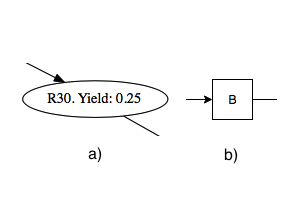
\includegraphics[scale=0.5]{Billeder/Reactions.png}
\caption{\textbf{a)} Reaction when part of output files from program. Consisting of "R"+ID and the yield of the reaction. \textbf{b)} Reaction when drawn as minor example for thesis. Always have capital letters as identifiers.}
\end{figure}
\subsection{Synthesis Plans}
A synthesis plan is a series of reactions that produces a target compound. The synthesis plans will usually have a reverse tree like structure where the root is the target compound and the leaves are starting compounds. All complete hypergraphs in this paper marks the target compound as red, and the starting compounds as green.
\begin{figure}[H]
\centering
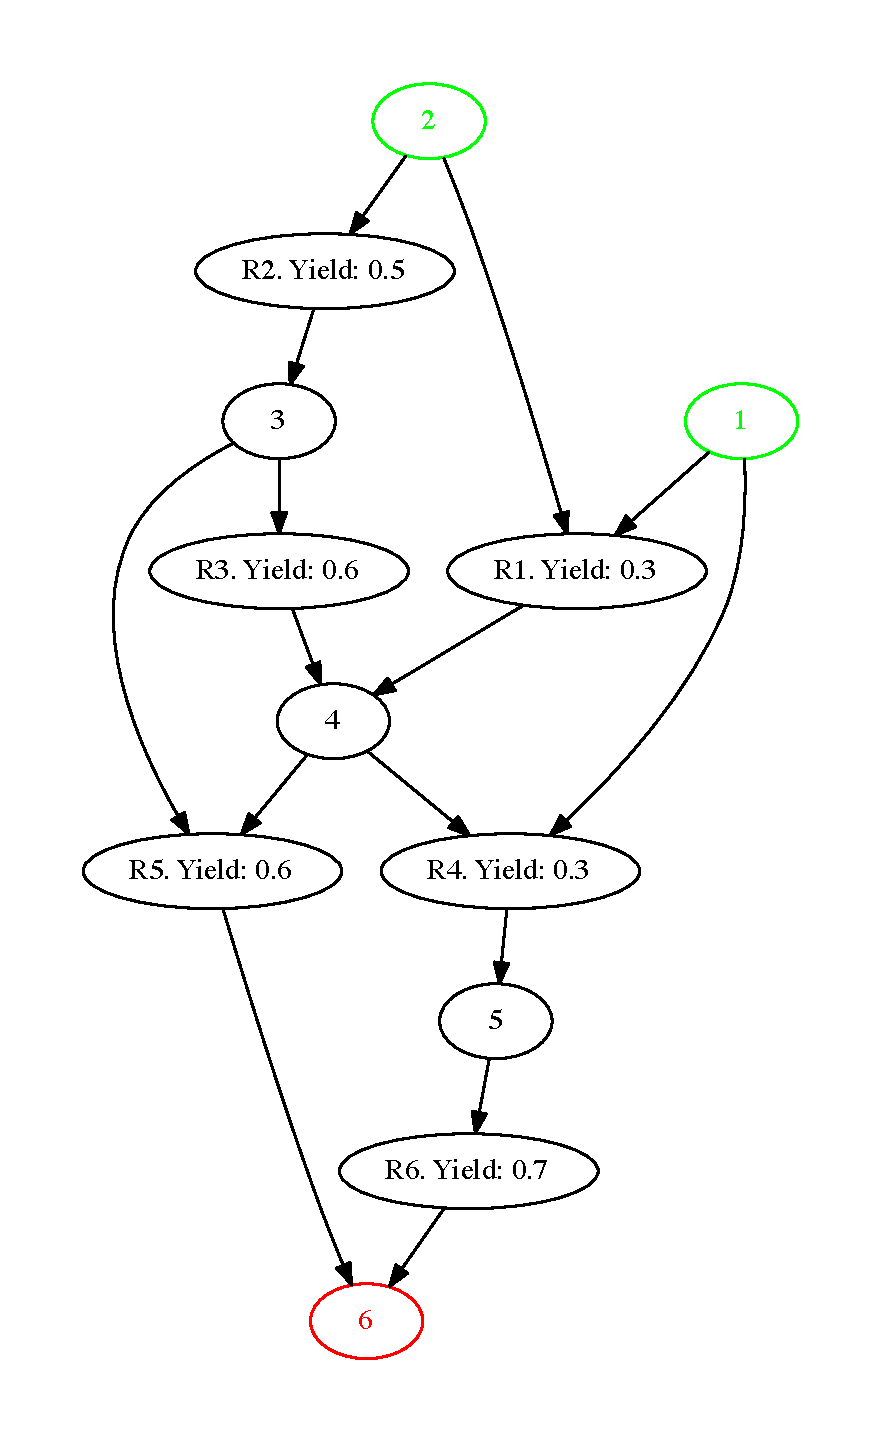
\includegraphics[scale=0.5]{TestGrafer/PaperTest.pdf}
\caption{Example of a complete hypergraph}
\label{fig::CompletegraphExample}
\end{figure}
When a synthesis plan is created the nodes are not colored. It is however easy to see that the compounds with in-degree = 0 is the starting compounds, and the only compound with out-degree = 0 is the target compounds.
\begin{figure}[H]
\centering
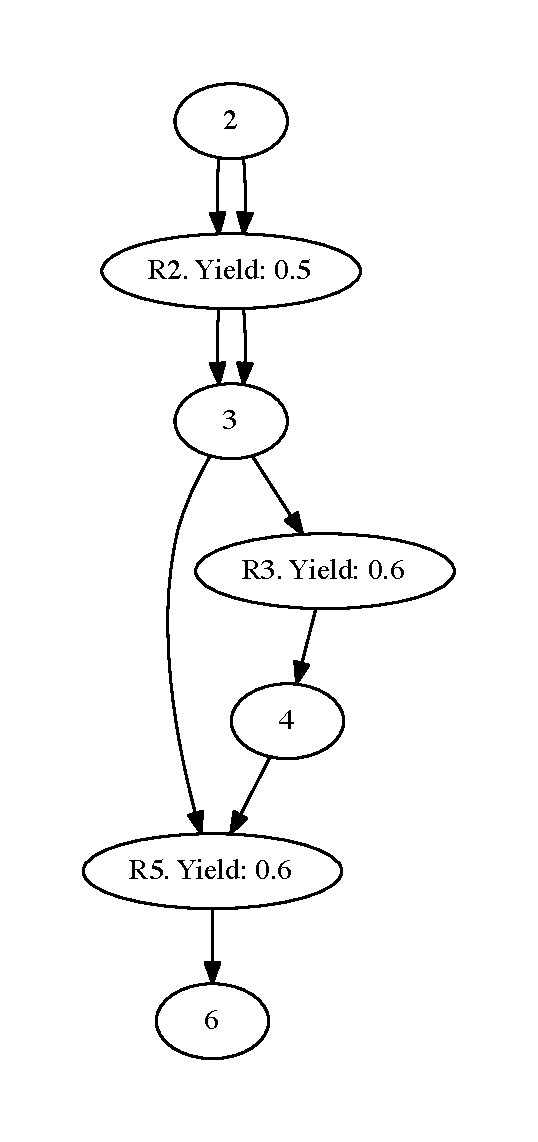
\includegraphics[scale=0.5]{Billeder/SynthplanExample.pdf}
\caption{Example of a synthesis plan given the hypergraph in fig. \ref{fig::CompletegraphExample} }
\end{figure}

\subsection{Hypergraphs and Hyperpaths}
\textbf{Hypergraphs}\\
A directed hypergraph $h$ is a set $V$ of vertices and a set $E$ of hyperedges, where each hyperedge $e=(T(e),H(e))$ is an ordered pair of non-empty multi-sets of vertices. The set $T(e)$ is denoted as the tail of the hyperedge and $H(e)$ is the head. If $|H(e)|=1$ then the hyperedge is denoted as a B-hyperedge. If all edges in the hypergraph is B-hyperedges, then the graph is denoted a B-hypergraph. This paper will only consider hypergraphs that are B-hypergraphs. A hypergraph $H' = (V',E')$ is a subhypergraph of $H=(V,E)$ if $V' \subseteq V$ and $E'\subseteq E$.\cite{Fagerberg}

\begin{figure}[H]
\centering
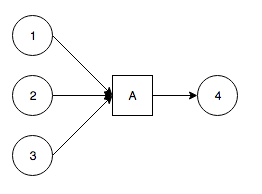
\includegraphics[scale=0.5]{Billeder/HyperEdge.png}
\caption{Example of hyperedge $A$. $T(A) = \{1,2,3\}$, $H(A) = \{4\}$}
\end{figure}

\textbf{Hyperpaths}\\
A path $P_{st}$ from $s$ to $t$ in a B-hypergraph is a sequence $P_{st}=\langle e_1, e_2, e_3, ... , e_q \rangle$ of B-hyperedges such that $s\in T(e_1)$ and $t=H(e_q)$ and $H(e_i) \in T(e_{i+1})$ for $i=1..q-1$. Its length $|P_{st}|$ is the number $q$ of hyperedges. If $t \in T(e_1)$, then $P_{st}$ is a cycle. A hypergraph is acyclic if it does not contain any cycles. \cite{Fagerberg} \\
A hyperpath $\pi_{st} = (V_{\pi},E_{\pi}$ from a source vertex $s$ to a target vertex $t$ in a B-hypergraph $H$ is a subhypergraph of H with the following properties: If $t = s$, the $V_{\pi}=\{s\}$ and $E_{\pi} = \emptyset$. Otherwise, $E_{\pi}$ can be ordered in a sequence $\langle e_1, e_2,....,e_q \rangle$ such that 
\begin{enumerate}
\item 
$T(e_i)\{s\} \cup \{H(e_1),h(e_2,...,h(e_i-1)\}$ for all i
\item
$t=H(e_q)$
\item
Every $v \in V_{\pi} \setminus \{t\} $ has at least one outgoing hyperarc in $E_{\pi}$, and $t$ has zero.
\item
Every $v \in V_{\pi} \setminus \{s\}$ has at least one ingoing hyperarc in $E_{\pi}$, and $s$ has zero. \cite{Fagerberg}
\end{enumerate}

\section{Designing a hypergraph in C++}
\label{sec::DesigningHyper}
A hypergraph consists of nodes and hyperedges. These where implemented as two structs that have their own seperate attributes.
\begin{figure}[H]
\centering
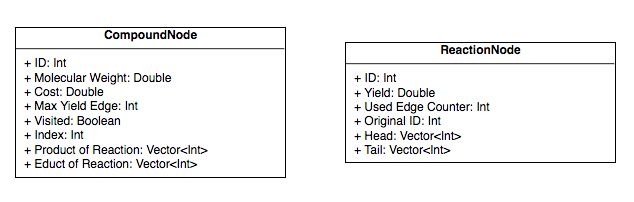
\includegraphics[scale=0.5]{Billeder/Compound-ReactionNode.png}
\caption{The structure of CompoundNodes (nodes) and ReactionNodes (hyperedges)}
\end{figure}
There are some non-trivial attributes in the CompoundNode struct.The difference between Molecular weight and the cost is that the cost is the accumulated weight of the given starting materials that is used to reach this compound, and the molecular weight is the actual weight the compound it self. This of course means that if a compound is a starting compound, then the cost and the molecular weight is the same.\\ The Max Yield Edge attribute is an identifier to the hyperedge that is used to reach this compound. The first time a compound is reached the attribute is changed to hold the ID of the reaction from where the algorithm came. If the compound is reached and the cost of the compound is changed, then the attribute would change, so that it always points to the edge used to calculate the current cost of the compound.\\
Visited and Index are attributes used when the hypergraph is pruned (Section \ref{Pruning}) and to keep track of a CompoundNodes position in the priority queue used when running STB-Dijkstra (Section \ref{STB-Dijkstra}).\\
The two vectors, Product of Reaction and Educt of Reaction, are lists containing information on which reactions the compound is a product of and which reactions it is a educt to. This is used to make traversal of the hypergraph easy.\\

The ReactionNode also contains some non-trivial attributes. The Used Edge Counter is used by the STB-Dijkstra algorithm (Section \ref{STB-Dijkstra}) to make sure that all educts to a reaction have had their min cost evaluated before the reaction can be used. The Original ID attribute is used when we need to change a hyperedge into a B-Hyperedge. If there is more than one product of a reaction we need to split the reaction into multiple new reactions, so that the hyperedge becomes legal. It is for result purpose needed to have a pointer to the original ID of the reaction.\\

The hypergraph is designed to consist of four dynamic lists, vectors, to facilitate quick lookup time and fast attribute reseting. The two vectors compoundList and reactionList are list of size $V$ and $E$ respectively, containing pointers to the compounds and reactions of the given hypergraph. These two vectors are used to reset the attributes of the compounds and reactions after each iteration of the algorithms. The compoundLookupList and reactionLookupList vectors are used to have have a constant lookup time at the cost of space. Both are vectors of pointers to compounds and reactions, just as compoundList and reactionList, but are of size $N$ and $M$ instead, where $N$ is the highest compoundID and $M$ is the highest reactionID. This means that if a reaction with ID 235406 is added to the hypergraph, a pointer to the reaction is pushed to to the back of reactionList and added to reactionLookupList[235406]. This makes it possible to edit a single compound or reaction in $\mathcal{O}(1)$ time, using the lookupLists, and to edit all compounds or reactions in $\mathcal{O}(|V|)$ and $\mathcal{O}(|E|)$ respectively.\\
If the structure was only used on homemade hypegraphs where we would label the compounds from $0,1, ... N$ and the reactions $0,1,...,M$, we would only need the two lookupLists, since we would have two vectors of size $V=N$ and $E=M$ and still have the constant lookup time. However, when working on real data we could have a hypergraph with the reactionIDs 6, 12820 and 50003829 as the only reactionsNodes in the hypergraph. This would result in a vector of size 50003829 but we only have three entries in the vector. So when we need to reset the attributes in the use of the shortest path algorithms we would have to run through the whole vector. This is where the two second lists are useful. Even though we have a reactionLookupList of size 50003829 the reactionList in this hypergraph would only be of size 3.
Notice that since we are working with pointers to, and not copies of, compoundNodes or reactionsNodes there is no problem in only changing the attributes by accessing it through one of the lists. 
\begin{figure}[H]
\centering
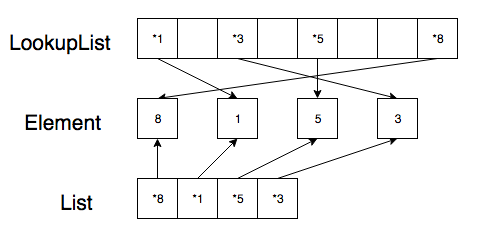
\includegraphics[scale=0.5]{Billeder/ListOverview.png}
\caption{Illustration of the difference between List and LookupList.}
\label{fig::ListLookupList}
\end{figure}
\section{Finding The K-Best Synthetic Plans}
\label{sec::K-Best}
This section describes how to find the K-Best paths of a hypergraph modifying an algorithm made by Jin Y. Yen. The section starts out by describing the work flow of the algorithm, and then proceeds to deal with the alterations that are needed to run the algorithm on a hypergraph.
\subsection{Yen's Algorithm}
Yen's algorithm is an algorithm that computes the K-shortest paths for a graph with non-negative edges. It was publish in 1971 and uses any shortest path algorithm to find the best path and then proceeds to find the $K-1$ deviation of the best path. \cite{Yen}

It starts out by finding the best path using a shortest path algorithm. Once the best path have been found it uses the path to find all the potential second best paths by fixing and removing edges in the graph. \\
By using the same first vertex as the original path but removing the first edge, it forces the shortest path algorithm to take another route through the graph and thereby creating a potential second best path. This is added to the list of potential paths and the algorithm can continue to derive other paths from the best path. By fixing the first edge in the previous best plan, Yen's algorithm forces the shortest path algorithm to take the first edge which it now shares with the best path. However, now the algorithm have removed the second edge from the original path and once again forces the shortest path algorithm to find alternative routes. This process is then repeated until we reach the next to last vertex in the best path.\\
By sorting the list of potential paths, it has the second best path at the start of the list and it can add it to the final list of best path. The algorithm then repeats on the second best path to find the third best path. This is done until all K-best path have been found or there are no more paths to find.
\subsection{Yen's Algorithm On Hypergraphs}
We use the principles from Yen's algorithm to make our own algorithm that will work on hypergraphs. To handle the problem of generating all derived paths from our best path in our hypergraph, we use a method called BackwardsBranching. \cite{Fagerberg} \cite{Nielsen} \cite{Carsten}
\begin{lstlisting} [emph={if,for, endif, endfor, function, endfunction, do}, emphstyle = \bfseries,caption = Backwards Branching for B-Hypergraph]
function Back-Branch(H,$\pi$)
	B=$\emptyset$
	for i = 1 to q do 
		Let H$^i$ be a new hypergraph
		H$^i$.V = H.V
		// Remove hyperarc from H
		H$^i$.E = H.E $\setminus \{\pi.p(v_i)\}$
		// Fix Back tree
		for j = i+1 to q do
			H$^i$.BS(vj) = \{$\pi.p(v_j)$\}
		B = B $\cup$ \{H$^i$\}
	return B
\end{lstlisting}
\begin{figure}[H]
\hspace{-2cm}
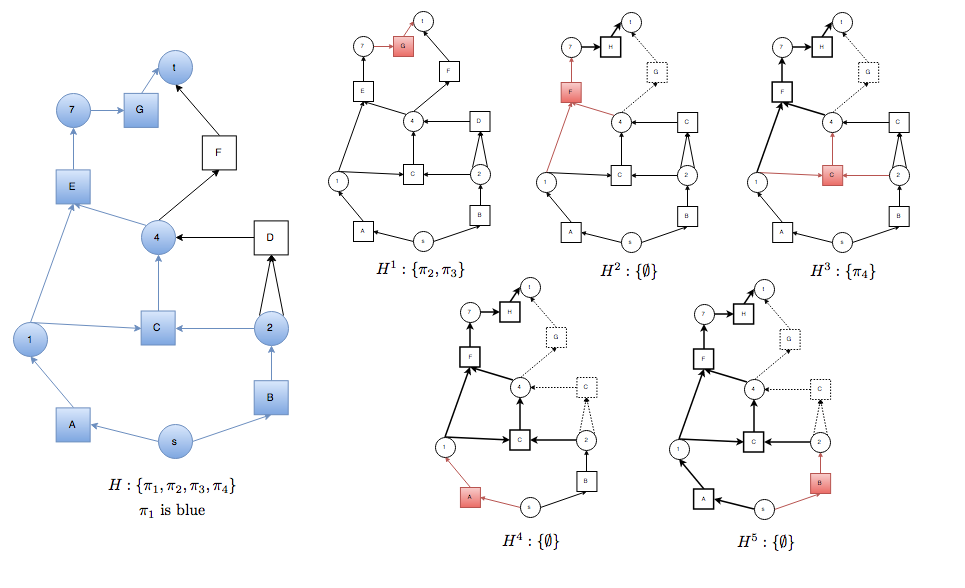
\includegraphics[scale=0.5]{Billeder/BachBranch}
\caption{An example of branching for hypergraphs. $H$ is the original hypergraph. The vertices and hyperedges marked with blue are part of the best path. The rest of the figure illustrates the backwards branching. Each of the smaller figures shows a hypergraph $H^i$ and how it is created from $H$. Dotted hyperedges and red heyperedges are not part of the hypergraph, but have been deleted due to branching. Hyperedges in bold are fixed hyperedges. When hyperedges are fixed it leads to other hyperedges being deleted (dotted). The caption beneath each hypergraph represents the possible paths that are available in the given hypergraph.}
\end{figure}
However, this algorithm have a problem when working on a larger hypergraph. It demands that each time we make alterations on the hypergraph we have to make a copy, $H^i$, of the graph, $H$, with the exception of the hyperedges that is removed when fixing the back tree and removing $\pi.p(v_i)$.\\
This could easily work for smaller graphs, but if we use this on a hypergraph that would contain all of the data from beilstein, we would have to copy a graph of multiple GigaBytes. \\
To handle this problem I came up with the idea of creating an overlay for the graph instead of copying it. The overlay would work as an transparent on top of the original graph, stating which edges still is accessible. This is done by creating a \textit{vector<bool>} which has a length of $R$, where $R$ is the number of reactions. Normally a reaction would contain at least 28 bytes of data:
\begin{itemize}
\item
3x ints of 4 bytes each
\item
1x double of 8 bytes
\item
1x \textit{vector<int>} head of length one of at least 4 bytes
\item
1x \textit{vector<int>} tail of length $N$ (number of educts) of at least 4 bytes
\end{itemize}
This can be reduced dramaticly by using the \textit{vector<bool>}, since c++ only uses 1 bit per boolean in the vector instead of the regular 1 byte per boolean.\cite{VectorBool} This means if working on a hypergraph with 40 million reactions, we would be able to create an overlay using 5 MB of space per alternated graph, instead of copying a hypergraph were the reactions alone uses at least 1,12 GB per copy. \\
As the figure below shows, we never change or remove anything on the hypergraph. We simply create the following overlay:
\begin{table}[H]
\centering
\begin{tabular}{c|c|c|c|c}
Reaction & A & B & C & D \\\hline
Usable & true & true & true & false \\\hline
Bit Representation & 1 & 1 & 1 & 0
\end{tabular}
\end{table} 
And then when trying to use an edge, we ask: "Does overlay at reaction A exist?". If yes, you can use it. If no, the edge have been "removed", and therefore cannot be used.
\begin{figure}[H]
\centering
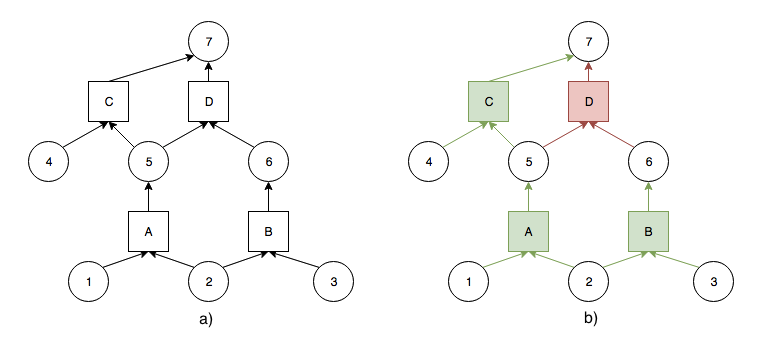
\includegraphics[scale=0.5]{Billeder/OverlayIllustration}
\caption{a) The original hypergraph. b) The original hypergraph, but using the overlay. If the reaction is green it is still usable. If red then it have been "removed" from the hypergraph.}
\end{figure}

This of course means that the algorithm for back-branch have to be changed accordingly. Instead of the hypergraph as input we now give it an overlay. This overlay is changed so it fits with the new layout of the graph. Instead of deleting hyperedges in the copy, we now simply changes the boolean at the index of the hyperedge.id. True if we should "add" the hyperedge and false when we want to "remove" a hyperedge.

\begin{lstlisting} [emph={if,for, endif, endfor, function, endfunction, do}, emphstyle = \bfseries,caption = Backwards Branching for B-Hypergraph using overlay]
function BackwardsBranching($\pi$, Overlay) 						
	List B = $\emptyset$
	// q = Path length
	for i = 1 to q do			
		//remove i'th hyperedge from Path in overlay					
		Set Overlay[$\pi$[i]] to false		
		//fix the backtree				
		for j = i downto 1	do							
			vertex C <- $\pi$[j].head
			for each hyperedge into C
				Set Overlay[reaction.id] to false
			Set Overlay[$\pi$[j]] to true
		endfor
		B = B $\cup $ {$Overlay$}
	endfor
	return B
endfunction
\end{lstlisting}
Now that we have the branching in place are we able to construct an algorithm that are similar to Yen's algorithm, but can run on hypergraphs. As input it takes a start node ($s$), a goal node ($t$), and an integer $K$, where $K$ is the number of best paths we want to find. The algorithm, however, only takes a single node as its starting node, which is a problem when working with hypergraphs. The reason for this is that the size of the tail of a hyperedge usually is larger than 1 and this by default gives us more than one starting node. This is fixed by making $s$ a dummy node that have an hyperedge $e = (H|1|, T|1|)$ to each of the starting nodes, transforming the multiple sources to a single source.\\
The algorithm creates a heap, $L$, and a list, $A$, which will contain the $K$-best paths once the algorithm is finished. It then finds the best path using a shortest path algorithm and inserts it into the heap. Inside the loop it extracts the best path found from the heap and performs a backward branching, and finds all possible paths in the branches. If there is a path from $s$ to $t$, then this path is added to the heap. The algorithm either terminates if the heaps is empty ( No more paths available) or once it have found the $K$-best paths.
\begin{lstlisting} [emph={if,for, endif, endfor, function, endfunction, do}, emphstyle = \bfseries,caption = K-Shortest Paths Algorithm in B-Hypergraph]
function YenHyp(s, t, K) 
	L = new heap with elements (overlay, $\pi$)
	A = List of shortest paths
	//(Graph is default overlay (all true))
	$\pi$ = shortestPath(Graph, s,t) 				
	Insert (Graph, $\pi$) into L
	for k = 1 to K do
		if L = $\emptyset$
			Break
		endif
		(Overlay$'$, $\pi'$) = L.pop
		add $\pi'$ to A
		for all Overlay$^i$ in BackwardBranching((Overlay$'$,$\pi'$)) do
			$\pi^i$ = shortestPath(Overlay$^i$, s, t)
			if $\pi^i$ is complete
				Insert( $H^i$, $\pi^i$) into L
			endif
		endfor
	endfor
	return A
endfunction
\end{lstlisting}
YenHyp makes $K$ iterations. In each iteration the length of a hyperpath determines the number of calls to the shortest path algorithm. The worst case for the length of the hyperpath is $\mathcal{O}(|V|)$. Hence the running time of YenHyp becomes:
\begin{equation}
\mathcal{O}(K \cdot |V| \cdot SP)
\end{equation}
Where $SP$ is the running time for the shortest path algorithm used.
\subsection{Cost Function}
Before we are able to find the K-best paths of our hypergraph, we should be able to compare them with each other. To do this we use a additive weight function defined in the following way on a given hyperpath $\pi_{st}$ from $s$ to $t$:

\begin{equation}
W(u)=\begin{cases}
    w(p(u)) + F(p(u)), & \text{if $u\in V\setminus \{s,\ starting\ nodes\}$}.\\
    C, & \text{Starting Nodes}. \\
    0, & \text{Otherwise}
  \end{cases}
\end{equation}

$W(u)$ define the cost of node $u$ and $C$ is in this particular case, the molecular weight of a compound. The predecessor function $p$ is used to find the hyperedge $e=p(u)$ which have $u$ as head. The function $F$ is a non-decreasing function of the sum of the weights of the nodes in the tail to $e$. Each of the nodes are multiplied by the retroyield of the edge, $1/yield$.

\begin{equation}
F(p(u)) = \sum(W(Tail(p(u)) \cdot (1/yield_{p(u)})
\end{equation}

We are now able to distinguish between the paths found and extract the K-best plans. \cite{Carsten}

\section{Shortest Path}
\label{sec::ShortestPath}
This section describes two different approaches to the shortest path problem in a hypergraph. A dynamic approach proposed by Carsten Grønbjerg Lützen and Daniel Fentz Johansen \cite{Carsten} and a Dijkstra inspired approach proposed by Lars Relund Nielsen, Kim Allan Andersen and Daniele Pretolani \cite{Nielsen}. 

\subsection{Dynamic Approach}
The dynamic approach to find shortest path in a hypergraph is an algorithm proposed by Carsten Grønbjerg Lützen and Daniel Fentz Johansen in their Master thesis \textit{A Computational and Mathematical Approach to Synthesis Planning}.\cite{Carsten}. It uses recursion to calculate the cost of compounds.

\subsubsection{Approach}
The dynamic approach starts at the target compound and moves away from it step by step in a recursive manner. Once it hits a starting compound it backtracks through the recursions, using the now gained cost to calculate the cost of those along its path. The approach can be defined as following:
\begin{equation}
Cost(V) = \displaystyle\min_{e\in productOfReaction} 1/yield_e \cdot \displaystyle\sum_{u\in Tail(e)} Cost(u)
\end{equation}
The cost of a node $V$ is the minimum over all the possible ways to synthesize it. The cost of a potential approach to synthesize node $V$ is the sum of cost of the educts involved times the retroyield of the reaction required for transforming the educts to the product V .\cite{Carsten}
	
\begin{lstlisting} [emph={if,for, endif, endfor, function, endfunction, do}, emphstyle = \bfseries,caption = Dynamic programming for finding the best path]
function Min(V)
	if(V) is starting material 
		return Cost of V
	endif
	mincost <- $\inf$
	for all $e\in BS(V)$ do
		cost <- cost of e
		for all $u \in Tail(e)$ do
			cost <- cost + Min(u)
		endfor
		if mincost $\leq$ cost 
			mincost <- cost
			V.minedge <- e
		endif
	endfor
	return mincost
endfunction
\end{lstlisting}

The worst hypergraph that we could run the algorithm on a hypergraph where each hyperedge $e=(|T| = 1, |H| = 1)$. When connected these would form a linked list which would lead to the running time of $\mathcal{O}(|V|+|E|)$. 
\begin{figure}[H]
\centering
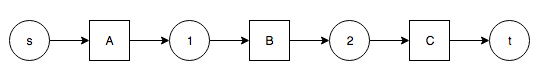
\includegraphics[scale=0.5]{Billeder/WorstCaseDynamic.png}
\caption{Example of worstcase scenario of a hypergraph}
\end{figure}


\subsubsection{Problems}
A problem with the dynamic approach is that it does not work on hypergraphs with cycles due to its recursive nature. When a cycle it hit, it will start an endless loop to figure out the cost of a node. 
\begin{figure}[H]
\centering
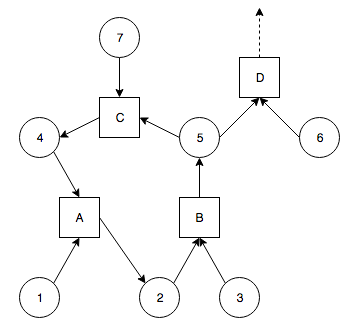
\includegraphics[scale=0.5]{Billeder/CycleGraph.png}
\caption{Example of graph with cycle.}
\label{fig::CycleGraph}
\end{figure}
As seen in the example in fig. \ref{fig::CycleGraph}, the algorithm enters the cycle in reaction D. When trying to calculate the weight of 5, it needs the weight of 2 and 3. 3 is a starting node, so the weight is the weight of the compound itself. 2 however needs the weight of 1 and 4. Again 1 is a starting node, so no calculations are needed. 4 however needs the weight from 7 and 5. Now we hit 5 again, and the loop starts. This could of course be handled by removing an edge from  the hypergraph, and thereby breaking the cycle. This however would effect the results, because how do we know that the edge we remove would not have contributed to a better result in the end. This is where Nielsen et. el STB-Dijkstra algorithm comes into play.
\subsection{The STB-Dijkstra Algorithm} \label{STB-Dijkstra}
Nielsen algorithm, or SBT-Dijkstra, is an algorithm that uses the same principles as shortest path algorithm conceived by Edsger W. Dijkstra in 1956. The original Dijkstra is asymptotically the fastest known single-source shortest-path algorithm for arbitrary directed graphs with unbounded non-negative weights. \cite{Dijkstra} Nielsen et. al. have modified it to be used on hypergraphs.
\subsubsection{Approach}
The algorithm requires that the cost of all nodes in the hypergraph is $\infty$ and that the hyperedge property $kj=0$. It then adds the dummy node $s$ to its priority queue. As long as the priority queue is not empty it will extract the minimum, and for each hyperedge going out of $u$ increase the $kj$ counter in the given hyperedge. Once the counter is equal to the size of the tail of the hyperedge, the algorithm can proceed to calculate the weight of the node $v$, which is the head of the hyperedge. Should the existing weight of $v$ be larger than the newly calculated weight, the algorithm updates the weight to the newly found weight and adds $v$ to the priority queue, given that the node have not been added from another edge. If the cost changes, the min-edge attribute is also set to be the edge from which the new cost have been calculated.
\begin{lstlisting} [emph={if,for, endif, while, endwhile, endfor, function, endfunction, do}, emphstyle = \bfseries,caption = STB-Dijkstra for finding the best path]
Initialization: Set W(u) = $\infty \ \forall\ u \in V$, $k_j = 0\ \forall\ e_j \in E$,$Q = \{s\}$ and $W(s)=0$
function SBT-Dijkstra
	while ($Q=\emptyset$) do
		select and remove $u\in Q$ such that $W(u) = min\{W(x)|x\in Q\}$
		for ($e_j \in FS(u)$) do
			$k_j <- kj+1$
			if ($k_j = |T(e_j)|$) 
				v <- h($e_j$)
				if (W(v) > w($e_j$) + F($e_j$))
					if ($v \notin Q$  
						Q <- Q $\cup$ \{v\}
					endif
					W(v) <- w($e_j$)+ F($e_j$)
					p(v) <- $e_j$
				endif
			endif
		endfor
	endwhile
endfunction
\end{lstlisting}
When node $u$ is removed from the candidate set $Q$ (the priority queue), $W(u)$ is the minimum weight of all hyperpath from $s$ to $u$. The condition in line 7 ensures that each hyperedge $e_j$ is processed only once after the minimum cost for its tail nodes have been determined. The implementation of the priority queue, $Q$, dictates the running time of the algorithm. I have followed Nielsen et. al. example and chosen a heap structure. Since I have decided to implement the simple binary heap the running time of the algorithm becomes: $\mathcal{O}(|E|\ log_2(|V|) + size(h))$. The size of the hypergraph, $h$, is the sum of the cardinalities of its hyperedges:

\begin{equation}
size(h) = \displaystyle\sum_{e\in E} |e|.
\end{equation}
Where the cardinality of a hyperedge $e$ is the number of nodes it contains, i.e. $|e| = |T(e)| + 1$.\cite{Nielsen}
\subsubsection{Optimizing For Large Hypergraphs}\label{Pruning}
Since the STB-Dijkstra algorithm expands to the whole graph it might check nodes that is not a part of the hyperpath we are looking for. If we look at the hypergraph in fig. \ref{fig::DeadEnd}, is it easy to see that given the starting nodes 1,2,3,4 and the goal 10, that there is no need to use the hyperedges R2, R4, and R8, since they never would lead to our goal.
\begin{figure}[H]
\centering
\includegraphics[scale=0.4]{Billeder/DeadEnd.pdf}
\caption{}
\label{fig::DeadEnd}
\end{figure}

I therefore decided to combine the dynamic approach with STB-Dijkstra algorithm. The dynamic approach starts at the goal node, and travel through the hypergraph until it reaches $s$, thereby only using nodes on the way from goal to start. The algorithm however had the problem of not being able to work on hypergraphs that contained a cycle, and we could not just delete an edge when we hit a cycle since it could lead to wrong results.\\
We can however use the dynamic algorithm to mark the edges it hits on the way from goal to start. This would make it able to detect when it hits a cycle, since the node would already have been marked, and simply just skip the node and proceed to the next in its potential path. Once the algorithm is finished, we can transform the markings to an overlay that limits the hypergraph so it only "consist" of the reactions hit by the dynamic algorithm. Using this overlay reduces the search space of the STB-Dijkstra from the whole hypergraph to only concern the hyperedges that will lead to a path from $s$ to $t$.
\begin{lstlisting} [emph={if,for, endif, while, endwhile, endfor, function, endfunction, do}, emphstyle = \bfseries,caption = Reduce STB-Dijkstra search space]
graphOverlay is a list of size = #hyperedges where all entries are false.
function reduceGraph(graphOverlay, v, s)
	if (v.id = s.id)
		return graphOverlay;
	endif
	if (v.visited = false) 
		for(reaction : v.ingoingEdge )
			for (tailCompound : reaction->tail) 
				v.visited <- true;
				graphOverlay = reduceGraph(graphOverlay, tailCompound, s);
			endfor
			graphOverlay[reaction.id] <- true;
		endfor
	endif
	return graphOverlay;
\end{lstlisting}
Since the running time for the dynamic approach was $\mathcal{O}(|V|+|E|)$, the combined running time becomes: 
\begin{equation}
\mathcal{O}((|V|+|E|)+(|E|\ log_2 (|V|) + size(h)))
\end{equation}
The $(V+E)$ is however removed since the $E\ log_2 (V) + size(h)$ dominates. This results in a running time of:
\begin{equation}
\mathcal{O}(|E|\ log_2 (|V|) + size(h))
\end{equation}
The reason that the terms $V$ and $E$ does not change since in worst case are we not able to prune any of the hypergraph away using the dynamic approach.
\subsection{Testing}
\label{sec::testing}
In the development phase of my implementation of the algorithms have I used some small instances of hypergraphs that would be easy to check if they were correct by running the algorithms by hand and check the results. The hypergraphs have previously been used in \cite{Carsten} (\ref{Appendix::ThesisGraph}) and \cite{Fagerberg} (\ref{Appendix::Paper Graph}). In this phase I also created small tests to check how the algorithms would handle cycles (\ref{Appendix::Cycle Graph}) and deadends (\ref{Appendix::DeadEnd Graph}).
However, to be able to test my implementations on a larger automated scale, I had my colleague Rojin Kianian use the program SynthWorker to create some random generated hypergraph. SynthWorker is the product of Carsten Grønbjerg Lützens and Daniel Fentz Johansens master thesis \cite{Carsten}. It have been tested thoroughly and can therefore be used to test the correctness of my implementations.
The smaller graphs, \ref{Appendix::Cycle Graph},\ref{Appendix::DeadEnd Graph}, \ref{Appendix::Paper Graph}, \ref{Appendix::ThesisGraph}, were all hardcoded in seperate testprograms, but when we started working with the automated test, we had to agree on a input format. We decided to go with a dot inspired format, which I already had used to visualize the hypergraphs and the output plans. The format contains of declarations and edges. It starts of by declaring all reactions and compounds. A compound is declared as following:
\begin{center}
ID, Identifier, notS/S, "Weight", Weight, "Cost", Cost;
\end{center}
An example could be the following compound: ID: 4, Weight = 5, Cost = 6,25, which is not a starting compound. This would be written in the input file as:
\begin{center}
4 N notS Weight 5 Cost 6.25 ;
\end{center}
The notS/S argument is to determine whether a compound is a starting compound (S) or a just a compound (notS).
As for a reaction the format should be:
\begin{center}
ID, Identifier, "Yield", Yield in decimal;
\end{center}
So the reaction with ID = 6 and a yield of 80 \% would be:
\begin{center}
6 R Yield 0.8 ;
\end{center}
As the reader might have guessed the "identifier" is either N or R, which tells us whether it is a compound = N or a reaction = R. The format then states that once all compounds and reactions have been declared, they should be followed by a line which separates the declarations and the edges. This line should always state "REACTIONS" to indicate that the following lines are edges. The connections between compounds and reactions are written in the regular dot notation: s->t. This creates an edge going from s to t. If s is an ID of a reaction, then it states that t is a part of s' tail. If t is an ID of a reaction, then s is a part of t's head. The example shows how reaction ID=3 is connected to its educts and products. The educts are compound ID=1 and compound ID=2 and the product is compound ID=0.
\begin{center}
0->3 ;\\
3->1 ;\\
3->2 ;\\
\end{center}
The test program written takes a hypergraph in the described format, the number of compounds and reactions, number of plans we wish (K) and a score table from SynthWorker. It then creates the hypergraph, tries to find $K$ best plans of the graph and the compares the results with those from the score table. To handle the minor issue of rounding errors a $\sigma$ can be assigned in the code. As of this moment $\sigma = 0,00007$. This constant have been chosen by running the tests with different values and noticing at what value the results became noticeable different.\\

\begin{table}[H]
\hspace{-2.5cm}
\begin{tabular}{|r|r|r|r|r|r|r|r|}
\hline
Test & Compounds & Reactions & Hypergraph & Plans existing & Plans found & Algorithm & \#Errors\\\hline
1 & 7 & 13 & \ref{Appendix::Rojin1} & 22 & 22 & Dynamic & 0\\\hline
1 & 7 & 13 & \ref{Appendix::Rojin1} & 22 & 22 & STB-Dijkstra & 0\\\hline
2 & 11 & 20 & \ref{Appendix::Rojin2}  & 20 & 20 & Dynamic & 0\\\hline
2 & 11 & 20 & \ref{Appendix::Rojin2} & 20 & 20 & STB-Dijkstra & 0\\\hline
3 & 8 & 14 & \ref{Appendix::Rojin3} & 22 & 22 & Dynamic & 0\\\hline
3 & 8 & 14 & \ref{Appendix::Rojin3} & 22 & 22 & STB-Dijkstra & 0\\\hline
4 & 40 & 128 & \ref{Appendix::Rojin4} & 476 & 476 & Dynamic & 17\\\hline
4 & 40 & 128 & \ref{Appendix::Rojin4} & 476 & 473 & STB-Dijkstra & 85\\\hline
5 & 13 & 46 & \ref{Appendix::Rojin5} & 2121 & 2121 & Dynamic & 5\\\hline
5 & 13 & 46 & \ref{Appendix::Rojin5} & 2121 & 2121 & STB-Dijkstra & 5\\\hline
6 & 206 & 1045 & \ref{Appendix::Rojin6} & 50 (limited) & 50 & Dynamic & 0 \\\hline
6 & 206 & 1045 & \ref{Appendix::Rojin6} & 50 (limited) & 50 & STB-Dijkstra & 0 \\\hline
7 & 35687 & 170002 & \ref{Appendix::Rojin7} & 50 (limited) & 50 & Dynamic & 0 \\\hline
7 & 35687 & 170002 & \ref{Appendix::Rojin7} & 50 (limited) & 50 & STB-Dijkstra & 0 \\\hline
\end{tabular}
\end{table}

As the table above shows, there is errors in the fourth and fifth test. However at a closer inspection the errors with the dynamic approach in test four and five and the errors with STB-Dijkstra in test five, are of minor concern since the problem is that the result is off by 0,0001. The 85 error in test four using STB-Dijkstra, is a misleading problem. The design of the test expects that the algorithms finds the same paths as SynthWorker. The problem is not that the STB-Dijkstra have found 85 wrong paths, but that it have only found 473 of the 476 path available. This means that each time a path is not found the path comparisons shifts by one, leading to faulty comparisons.\\

Why the STB-Dijkstra algorithm fails to find the three missing paths is a problem that have not been solved. It is suspected to have something to do with the priority queue implemented and the ordering of the nodes within. There are a lot of error prints from the decrease-key function, stating that the key given is not smaller than the one already existing. These errors have only been seen when running on the tests from Rojin, and I suspect that it is because there are many paths with the same cost, and that this leads to some problems in the if statements that checks whether a newly calculated cost is lower than the existing, thus leading to a potential false instead of true.

\section{Beilstein Data}
\label{sec::BeilsteinData}
The Beilstein database is the largest database in the field of organic chemistry. Since 2009, the content has been maintained and distributed by Elsevier Information Systems in Frankfurt under the name "Reaxys".
The content covers more than 200 years of chemistry and has been abstracted from several thousands of journal titles, books and patents. Today the data is drawn from selected journals (400 titles) and chemistry patents, and the extraction process for each reaction or substance data included needs to meet three conditions:
\begin{enumerate}
\item
It has a chemical structure
\item
It is supported by an experimental fact (property, preparation, reaction)
\item
It has a credible citation
\end{enumerate}
Journals covered include \textit{Advanced Synthesis and Catalysis, Angewandte Chemie, Journal of American Chemical Society, Journal of Organometallic Chemistry, Synlett} and \textit{Tetrahedron}. \cite{WikiReaxys}\cite{WikiBeilstein}
\subsection{Data Access}
As mentioned above the content of the database is maintained and distributed by Elsevier Information Systems under the name "Reaxys". Reaxys\footnote{https://new.reaxys.com/} is accessible through any browser and is easy to navigate. It is possible to find a compound or a reaction and locate all the documents in which they have been a part of. An example would be the compound Strychnidin-10-one which is referenced in 1442 documents. This is also possible the other way around. Through Reaxys is it possible to search for a specific paper using keywords, authors, publication year, Journal title, etc. Once the paper have been found it is possible to see reactions and compound that are connected to this particular article. All data connected to a article, reaction or compound can be exported and downloaded through the Reaxys interface in different formats. In this thesis I have used the XML format to extract data from the database. It is important to notice that to use Reaxys properly, a login is required. I have here used the "sign in by your institution" function, making it possible to use the WAYF (Danish Universities and Higher Education) as a login.
\subsection{Data Assessment}
\label{sec::Assesment}
During my work with the data from the Beilstein database have I found several issues when it comes to using it to find shortest paths.
First problem is that there are multiple instances of the same compound, each with a different Reaxys IDs. As seen in fig.\ref{fig::SameID} have I found four different IDs for the compound Dysidiolide. These were found when I tried to reproduce the different synthesis plans of Dysidiolide from \cite{SynthesisPlans} using the referenced articles where each synthesis plan origins. E. J. Corey's version of Dysidiolide have the ID 8171938, Boukouvalas have two different with ID 7601810 and 7910427 and Danishefsky have the ID 7910428. \\
Since we have four different IDs for Dysidiolide we can't state a single goal compound to our program that would result in giving us these three synthesis plans. To handle this problem the program can take several goal compounds as an input, and by creating a dummy node $t$ are we able to give the illusion of a single target.

\begin{figure}[H]
\hspace{-1cm}
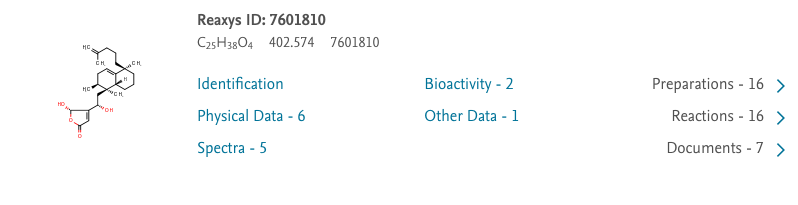
\includegraphics[scale=0.5]{Billeder/Dysidiolide-7601810.png}

\hspace{-1cm}
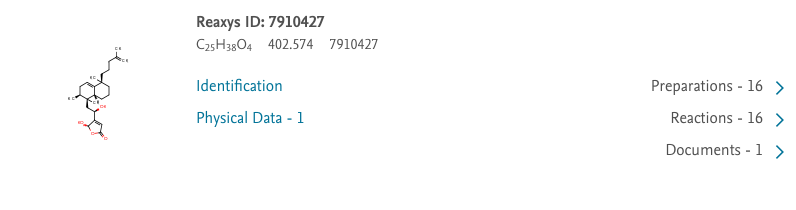
\includegraphics[scale=0.5]{Billeder/Dysidiolide-7910427.png}

\hspace{-1cm}
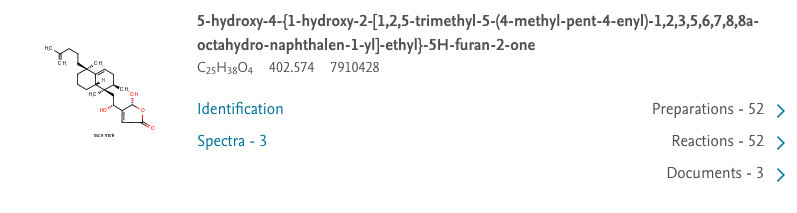
\includegraphics[scale=0.5]{Billeder/Dysidiolide-7910428.png}

\hspace{-1cm}
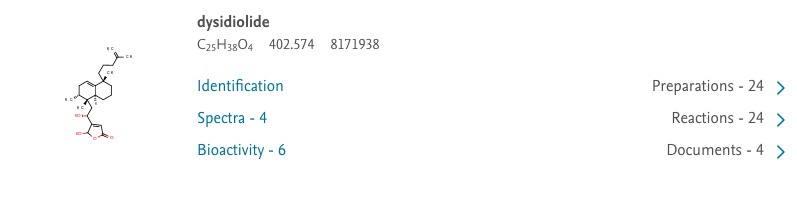
\includegraphics[scale=0.5]{Billeder/Dysidiolide-8171938.png}
\caption{Four different instances of Dysidiolide in Reaxys.}
\label{fig::SameID}
\end{figure}

So what is causing this multiple ID issue? If we study fig. \ref{fig::SameID} can we see that the molecular weight and molecular formular are exactly the same, however if we look at the close up of the molecular structure in fig. \ref{fig::SameIDClose} the compounds are not structured in the same way, even though the compounds are the same. The main differences is:
\begin{enumerate}
\item
Which way some of the substructures are facing. Example: The lower $C_4O_3H_4$ is rotated differently in each instance or that we write $H_2C$ instead of $CH_2$.
\item
How the bond between two chemical elements are notated. Example: The bond to the $OH$ in the bottom of the structure is either a "single" (d), "single down" (a) (c) or "single up or down" (b).
\end{enumerate}

\begin{figure}[H]
\begin{subfigure}{.5\textwidth}
  \centering
  \vspace{0.4cm}
  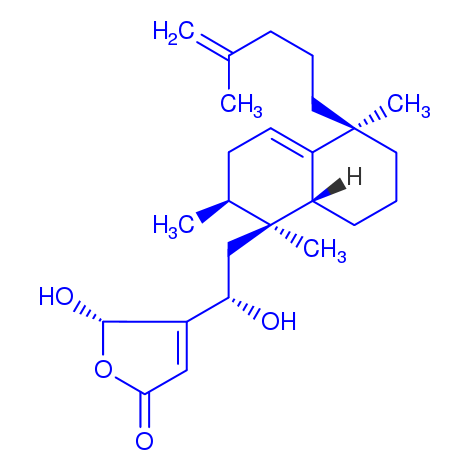
\includegraphics[width=.8\linewidth]{Billeder/Dysidiolide-7601810-Close.png}
  \vspace{1.3cm}
  \caption{}
\end{subfigure}%
\begin{subfigure}{.5\textwidth}
  \centering
  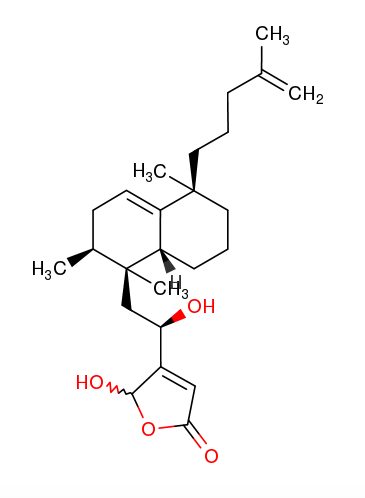
\includegraphics[width=.8\linewidth]{Billeder/Dysidiolide-7910427-Close.png}
  \caption{}
\end{subfigure}
\begin{subfigure}{.5\textwidth}
  \centering
  \vspace{0.4cm}
  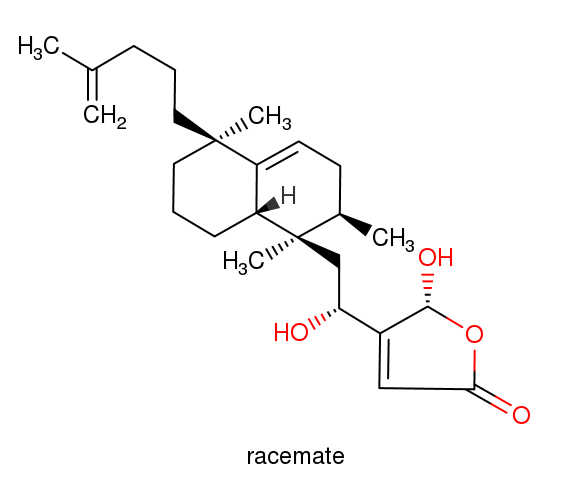
\includegraphics[width=.8\linewidth]{Billeder/Dysidiolide-7910428-Close.png}
  \vspace{1.3cm}
  \caption{}
\end{subfigure}%
\begin{subfigure}{.5\textwidth}
  \centering
  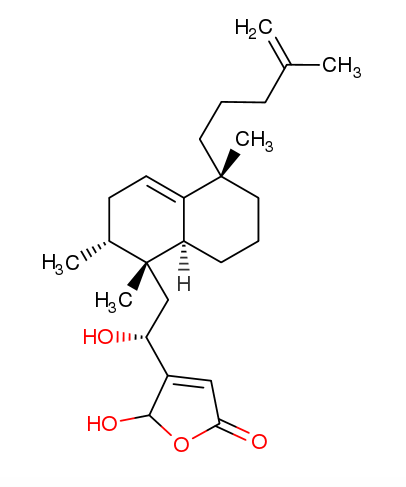
\includegraphics[width=.8\linewidth]{Billeder/Dysidiolide-8171938-Close.png}
  \caption{}
\end{subfigure}
\caption{Different versions of Dysidiolide: (a) ID 7601810 , (b) ID 7910427, (c) ID 7910428,  (d) ID 8171938}
\label{fig::SameIDClose}
\end{figure}

Second issue is the problem of a reaction not having an educt or a product(fig: \ref{fig::EductProductMissing}). This leaves the reaction incomplete and makes it useless in the graph construction. If there is no educt the hyperedge created will have an indegree of 0, and thereby making it unreachable. If there is no product the hyperedge will have an outdegree of 0, making it a deadend.

\begin{figure}[H]
\hspace{-1cm}
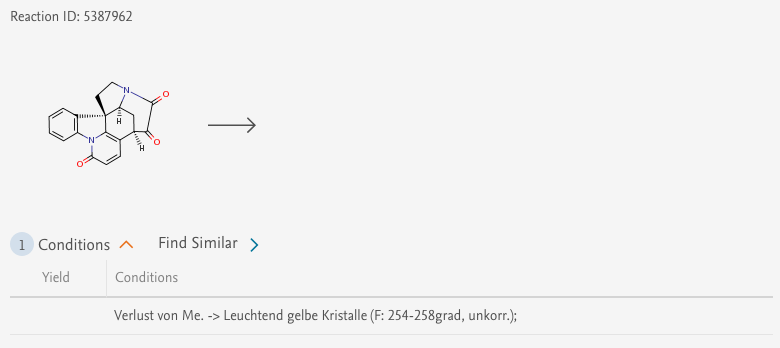
\includegraphics[scale=0.5]{Billeder/LeftOnlyReaction.png}

\hspace{-1cm}
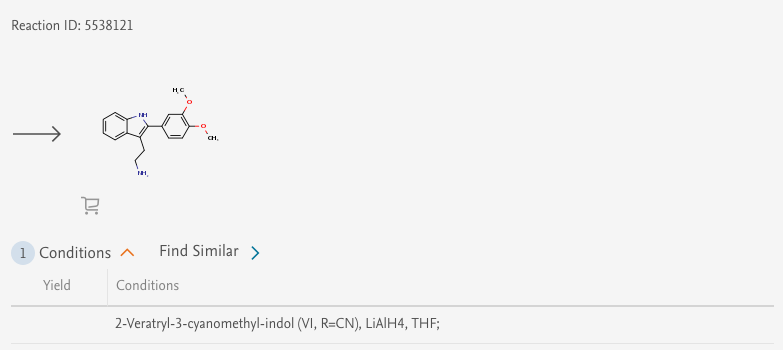
\includegraphics[scale=0.5]{Billeder/RightOnlyReaction.png}
\caption{Example of reactions that either is missing educts or products.}
\label{fig::EductProductMissing}
\end{figure}

Third issue is that some reactions contains educts where a compound isn't linked to a compound in the database. This results that the name of the compound is written instead of the usual structure diagram (fig \ref{fig::NoCompound}). This issue does not give problems when it comes to the construction of the hypergraph. The compound is simply just not added to the hypergraph. This however results in a slightly misleading result if the user does not look up the reaction in Reaxys where the name of the educt is stated. Example: If $A+B\rightarrow C$ but $B$ is not given an compound ID the reaction would look like $A\rightarrow C$ in the hypergraph.

\begin{figure}[H]
\hspace{-1cm}
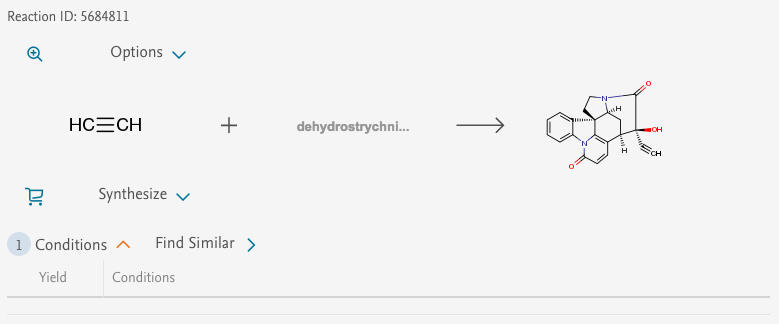
\includegraphics[scale=0.5]{Billeder/MissingIngredientReaction.png}
\caption{Example of an reaction with a missing educt.}
\label{fig::NoCompound}
\end{figure}

Forth issue is multireactions. (fig \ref{fig::Multistep}) A mulitreaction is a reaction with its own ID, but it consists of an educt and a product were there are multiple reaction steps, $s$, between the two compounds. This means that instead of $s$ different reactions with their own ID and yield we get a single reaction without a yield. The yield for each reaction in the multistep reaction is often stored as a part of the reaction text, but not easy extractable. The multistep reaction should however only consist of individual reactions that already are in the database.\\
The solution to this problem have been to not include all reactions labelled as "Multi-step reaction" when trimming the XML files from Reaxys. Since the steps should be saved as individual reactions this would not cause any harm to possibility of finding the exact same path, but only using all $s$ steps instead of one.

\begin{figure}[H]
\hspace{-1cm}
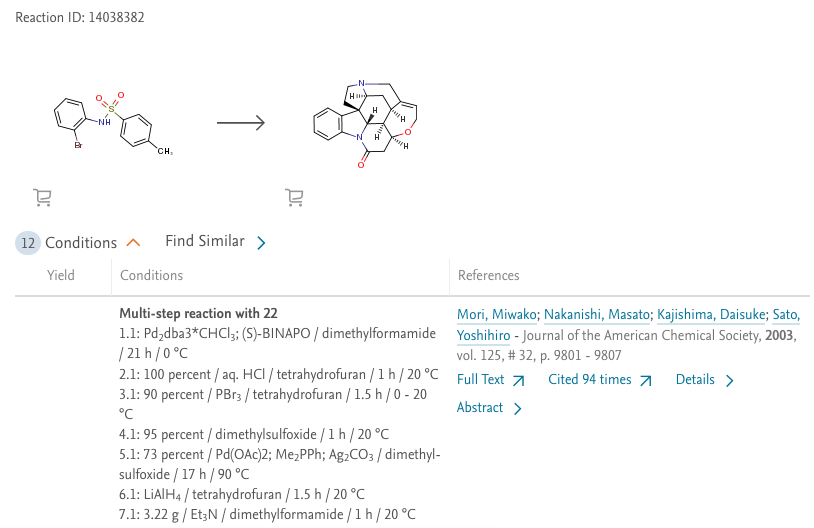
\includegraphics[scale=0.5]{Billeder/MultistepReactions.png}
\caption{Example of a multistep reaction.}
\label{fig::Multistep}
\end{figure}

\begin{figure}[H]
\hspace{-1cm}
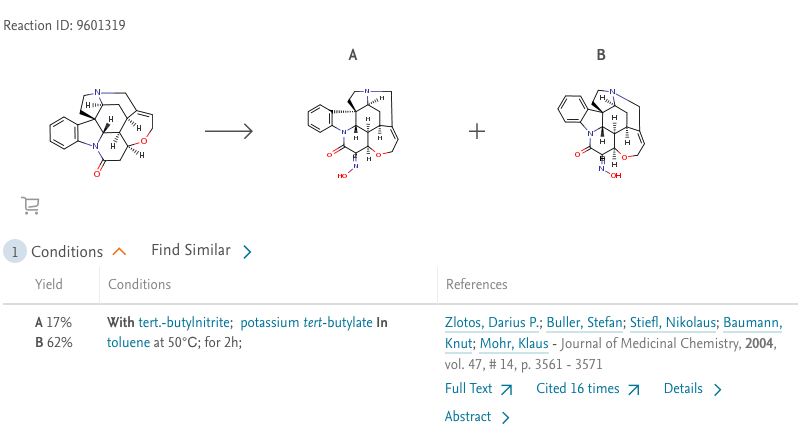
\includegraphics[scale=0.5]{Billeder/MultipleProducts.png}
\caption{Example of a reaction with multiple products}
\label{fig::MultipleProducts}
\end{figure}
\label{ConvertToB-Hypergraph}
Fifth issue is reactions which have more than one product (fig. \ref{fig::MultipleProducts}). If this becomes a part of our hypergraph it is no longer a B-hypergraph. This is a problem since both shortest paths algorithms only works on B-hypergraphs. This problem is however solved after the graph have been created by the method $convertToBHypergraph()$ in Hypergraph.hpp. The method iterates through the reaction list and if it encounters a non B-hyperedge, the hyperedge is added to a list of non B-hyperedges. For each of the non fixed B-hyperedges, $e$, it creates $|H(e)|$ new hyperedges, $e_i$, where $T(e_i)=T(e)$ and $H(e_i) = H(e)[i], \forall\ i \in \mathbb{N}, 1 \leq i\leq|H(e)|$  (fig. \ref{fig::CopyReaction}). Each of the new reactions contains an original-ID variable that points to the original hyperedge. This is only used to print the correct ID when the edge is used in a synthesis plan.

\begin{figure}[H]
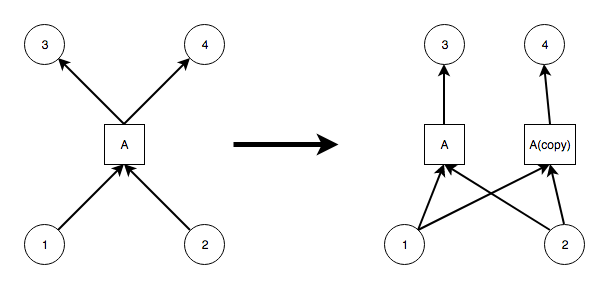
\includegraphics[scale=0.5]{Billeder/CopyReaction.png}
\caption{Convertion to B-Hyperedge}
\label{fig::CopyReaction}
\end{figure}

\section{Experiments and Results}
\label{sec::Results}
This section seeks to prove the usefulness of the K-best synthesis plan algorithm. This is done by using data from Beilstein based on already known synthesis plans in the pursuit of recreating these exact synthesis plans using the K-best synthesis plan algorithm.
\subsection{Idea and data extraction}
To prove that the k-best synthesis plan algorithm have a practical use in the real world, it should be able to create synthesis plans based on real data from the Beilstein database, and not just home made hypergraphs. There are however multiple problems with this:
\begin{enumerate}
\item
How do we choose the target compound and staring materials
\item
How do we validate the output?
\item
Direct access to the Beilstein database in Leipzig is not allowed
\end{enumerate}
The answer to 1 and 2 are automatically combined. The first part of 1 "How do we choose the target compound?" could be  answered as trivially as: Any random compound in the world. This of course leads to the second part: How do we then choose were to start. If the target compound is random then there is no way to know where a non-naive starting point would be, without having the theoretical and practical knowledge of a chemist. With a non-naive starting point I mean a starting material that is not the target material it self or the tail of the reaction to which the target is the head. Suppose that we where able to choose a random target and even assign some starting materials that would lead to a set of synthesis plans, how would we then validate these plans?\\
So instead of picking starting compounds and target compound in the dark, I chose to use already described synthesis plans as input when creating the hypergraphs. Hoffmann\cite{SynthesisPlans} have in his book "Elements of Synthesis Planning" described multiple synthesis plans of different compounds with correct citation to the articles in which they have origin. By using this book, I would be given the target compound and the corresponding starting materials. Furthermore I would have the already known synthesis plans to validate some if not all results of the K-best algorithm. The compounds that are described in the book is: Strychnine with 9 plans, Colchicine with 5 plans, Dysidiolide with 4 plans, Asteriscanolide with 4 plans and Lepadiformine 4 plans.\\

As for the problem with no direct access to the Beilstein database is there a simple solution. As mentioned before the browser interface Reaxys allows the user to export and thereby extract data from the database in a limited sense. It will not allow a full download of all 48 million compounds and their corresponding reactions with a single click, but it will allow to download XML files containing the information of single compounds, reactions and most importantly articles. As mentioned in section \ref{sec::BeilsteinData} the XML file of an article holds the ID of all reactions and the ID of the compounds that are part of these reactions. This means that it is possible to search for each of the synthesis plans from Hoffmann, using the article as a reference, and thereby download articles information in the XML file. This XML file should then contain all the reactions and compounds that are needed to recreate this particular synthesis plan.\\
The file contains a lot more information than needed to create a hypergraph so the file would have to be trimmed in order to be useful. The snippet below show one of the most important parts of the XML file.

\begin{lstlisting}[numbers=none]
<RX>
	<RX.ID>406669</RX.ID>
	<RX01>
		<RX.RXRN>1209486</RX.RXRN>
		<RX.RCT>glyoxylic acid ethyl ester</RX.RCT>
	</RX01>
	<RX01>
		<RX.RXRN>296858</RX.RXRN>
		<RX.RCT>2-[2-(3,4-dimethoxyphenyl)-1H-indol-3-yl]
				-ethylamine</RX.RCT>	
	</RX01>
	<RX02>
		<RX.PXRN>354389</RX.PXRN>
		<RX.PRO>{2-[2-(3,4-dimethoxy-phenyl)-indol-3-yl]
				-ethylimino}-acetic acid ethyl ester</RX.PRO>
	</RX02>
\end{lstlisting}
This is one of the reactions that is part of a synthesis plan for strychnine. 
\begin{itemize}
\item
<RX.ID> defines the reaction ID
\item
<RX01> defines the educt(s) of the reaction.
\item
<RX02> defines the product(s) of the reaction.
\item
<RX.RXRN> contains the ID of the compound in play.
\end{itemize}
So as the XML file states above, the reaction with ID: 406669 looks like this
\begin{equation}
296858 + 1209486 \rightarrow 354389
\end{equation}
Many of the reactions also contains the field <RX.MYD>. This is the yield of the reaction in percentage. Another important field is <RX.RTYP> that defines what type of reactions is it. Here we want to filter out all those saying "Multi-Reaction" since they cannot be used in the hypergraph construction. As mentioned in \ref{sec::BeilsteinData} this should however not interfere with the results since each reaction in a multi-step should also be saved as an individual reaction.\\

Since it would not make much sense to find a synthesis plan in a hypergraph consisting of only that particular synthesis plan, I decided to extract the XML files of each of the articles connected to a particular target compound, and combining them all into a single hypergraph that should contain all the synthesis plans to that single target compound. 
\subsection{Strychnine}
There are in Hoffmann\cite{SynthesisPlans} nine different plans for the compound Stychnine. These synthesis plans have published in the following articles:
\begin{itemize}
\item
R. B. Woodward, M. P. Cava, W. D. Ollis, A. Hunger, H. U. Daeniker, K. Schenker,
Tetrahedron 1963, 19, 247-288.
\item
V. H. Rawal, S. Iwasa, J. Org. Chem. 1994, 59, 2685-2686.
\item
S. D. Knight, L. E. Overman, G. Pairaudeau, J. Am. Chem. Soc. 1993, 115,
9293-9294.
\item
M. J. Eichberg, R. L. Dorta, K. Lamottke, K. P. C. Vollhardt, Org. Lett. 2000, 2,
2479-2481.
\item
G. J. Bodwell, J. Li, Angew. Chem., Int. Ed. 2002, 41, 3261–3262. (Angew. Chem.
2002, 114, 3395-3396).
\item
D. Solé, J. Bonjoch, S. Garcia-Rubio, E. Peidró, J. Bosch, Angew. Chem. Int. Ed.
Engl. 1999, 38, 395-397. (Angew. Chem. 1999, 111, 408-410)
\item
M. Mori, M. Nakanishi, D. Kajishima, Y. Sato, J. Am. Chem. Soc. 2003, 125,
9801-9807.
\item
Y. Kaburagi, H. Tokuyama, T. Fukuyama, J. Am. Chem. Soc. 2004, 126,
10246-10247.
\item
T. Ohshima, Y. Xu, R. Takita, M. Shibasaki, Tetrahedron 2004, 60, 9569-9588.
\end{itemize}
The article by T. Ohshima, Y. Xu, R. Takita, M. Shibasaki was however not to be found through Reaxys. The extracted hypergraph consisted of 459 compounds and 296 reactions. Out of these 296 reaction, only 190 of them were remaining in the final hypergraph. This is because all non-educt or non-product reactions were removed.
\begin{figure}[H]
\centering
\includegraphics[scale=0.03, angle=90]{Synteseplaner/Strychnine/Output.pdf}
\caption{Small version of the hypergraph. \href{Synteseplaner/Strychnine/Output.pdf}{Press here to see full pdf}}
\end{figure} 
As it can be seen the right part of the hypergraph consists of many non-linked single or small step reactions. It is assumed that the links between these reactions and between the rest of the hypergraph are missing because:
\begin{itemize}
\item
The reaction that connected two parts were a multi step reaction, and there was no single step reaction described in the articles.
\item
The links were there but because they were not correctly saved in Beilstein they had become non-educt or non-product reactions, which have been delete.
\item
The articles do in fact describe the reaction, but it is only mentioned as a reference to another article. It is possible that reactions not properly described the article, but only referenced, may not be saved in the XML file.
\end{itemize}
Despite the lack of connectivity of the hypergraph, the K-best algorithm was still able to find 16 different synthesis plans. This is impressive taken into account that we only used 8 plans to create the hypergraph.
\begin{table}[H]
\centering
\begin{tabular}{|r|r|r|}
\hline
Plan & Reactions & Starting weight \\ \hline
1 & \ref{Appendix::Strychnine1} & 2471,93 \\\hline
2 & \ref{Appendix::Strychnine2} & 3941,73 \\\hline
3 & \ref{Appendix::Strychnine3} & 4577,65 \\\hline
4 & \ref{Appendix::Strychnine4} & 5871,33 \\\hline
5 & \ref{Appendix::Strychnine5} & 6076,83 \\\hline
6 & \ref{Appendix::Strychnine6} & 8186,61 \\\hline
7 & \ref{Appendix::Strychnine7} & 8558,73 \\\hline
8 & \ref{Appendix::Strychnine8} & 13054,3 \\\hline
9 & \ref{Appendix::Strychnine9} & 13647,7 \\\hline
10 & \ref{Appendix::Strychnine10} & 19444,8 \\\hline
11 & \ref{Appendix::Strychnine11} & 20125,4 \\\hline
12 & \ref{Appendix::Strychnine12} & 20328,7 \\\hline
13 & \ref{Appendix::Strychnine13} & 21040,2 \\\hline
14 & \ref{Appendix::Strychnine14} & 21587,3 \\\hline
15 & \ref{Appendix::Strychnine15} & 44400,5 \\\hline
16 & \ref{Appendix::Strychnine16} & 277503 \\\hline
\end{tabular}
\caption{}
\label{tab::StrychnineResults}
\end{table}
So what is going on? When looking at the plans that was found and match them with the synthesis plans of Hoffmann, it became clear that plan 1-13 all have their offset in the synthesis plan by K. P. C. Vollhardt (fig. \ref{fig::Vollhardt}). The first 5 plans all contain the same compounds, but are different in the reactions they use. This is quite interesting since this shows how large an impact the choice of reactions have in a synthesis plan. During those 5 plans the accumulated weight of the starting compounds have more than doubled.\\
Plan 6-13 are almost the same story as 1-5. Each new plan switches a single reaction, and every second plan decides that it would be better to add the intermediate step of creating compound 8657520 instead of changing a reaction.
\begin{figure}
\centering
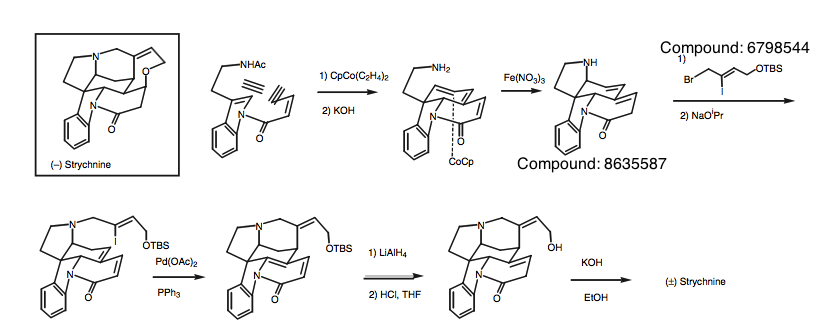
\includegraphics[scale=0.5, angle=90]{Synteseplaner/Strychnine/Vollhardt.png}
\caption{Strychnine synthesis by K. P. C. Vollhardt \cite{SynthesisPlans}}
\label{fig::Vollhardt}
\end{figure}
What the first 13 plans of strychnine shows is that it is hard to match the plans with the synthesis plan from Hoffmann. The synthesis plan (fig. \ref{fig::Vollhardt}) pictured in Hoffman only matches on the lower part of the generated synthesis plans. Compound 8635587 is the last compound that can be matched with a compound in the synthesis plan in Hoffmann. The top of the graph only concerns the synthesis of compound 6798544 which is a part of a larger reaction in the synthesis plan by Vollhardt.\\
\begin{figure}
\centering
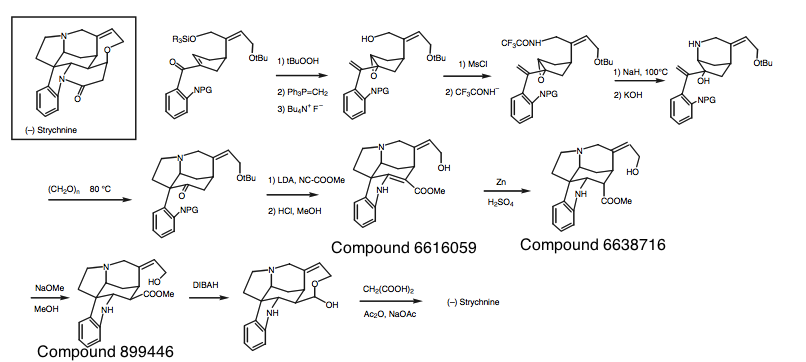
\includegraphics[scale=0.5, angle=90]{Synteseplaner/Strychnine/Overman.png}
\caption{Strychnine synthesis by L. E. Overman \cite{SynthesisPlans}}
\label{fig::Overman}
\end{figure}

\begin{figure}
\centering
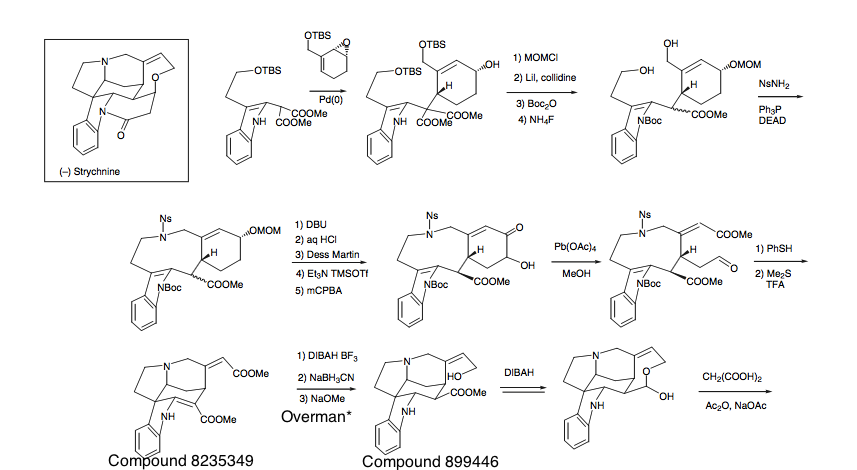
\includegraphics[scale=0.5, angle=90]{Synteseplaner/Strychnine/Fukuyama.png}
\caption{Strychnine synthesis by T. Fukuyama \cite{SynthesisPlans}}
\label{fig::Fukuyama}
\end{figure}

\begin{figure}
\centering
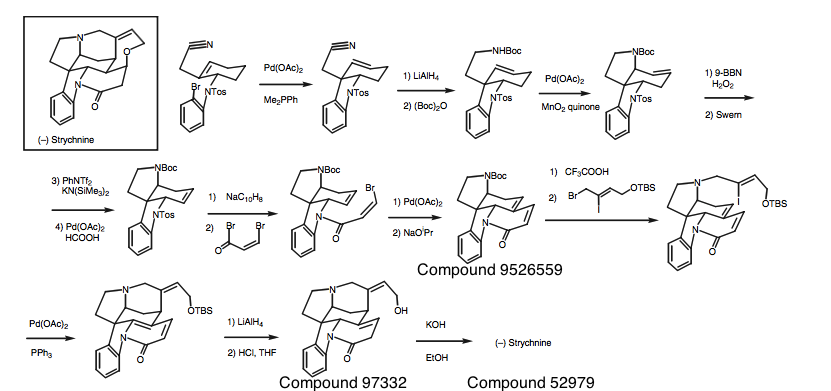
\includegraphics[scale=0.5, angle=90]{Synteseplaner/Strychnine/Mori.png}
\caption{Strychnine synthesis by M. Mori \cite{SynthesisPlans}}
\label{fig::Mori}
\end{figure}
Plan 14 seems to be a merge of the synthesis plan from L. E. Overman (fig. \ref{fig::Overman}) and the plan of T.Fukuyama (fig. \ref{fig::Fukuyama}). The step between compound 8235349 and compound 899446 in Fukuyama expands to contain two more reactions that passes through compound 6616059 and compound 6638716, that both are part of Overmans synthesis plan. I suspect that since Overman published his synthesis plan in 1993 and Fukuyama published his in 2004, Fukuyama has used these reactions when creating his own synthesis plan.\\

Plan 15 and 16 are both from the synthesis plan of Mori (fig. \ref{fig::Mori}). The only difference of these two plans is where they stop. This is due to the fact that the compound 97332 ((+)-isostrychnine) is the stage before compound 52979 ([3H]-Strychnine), but both have been given as goal compounds. This of course means that since 97332 is reached first, it becomes a better plan than 52979 which requires an extra reaction.\\

When looking at the results in tab. \ref{tab::StrychnineResults} it might be weird that last 3 plans have such a high starting weight taking into consideration that they are from other plans than the 13 first and that both Mori and Fukuyama are newer publications. Would it not be assumed that they should be better then? The thing is they all have had a reaction which had no yield in the XML files are therefore have been assigned a yield automatically of 10 \%. This of course is not acceptable when trying to find the best paths available, but bare in mind that the goal of these experiments was not to find the best plans, but to find the plans and validate them with already known synthesis plans. If the data set had been fulfilling the scores would have been better - at least on plan 14 and 15. Plan 16 has a quite expensive last reaction from compound 97332 to 52979 with a yield of only 16\%.
\subsection{Colchicine} 
There are in Hoffmann\cite{SynthesisPlans} five different plans for the compound Colchicine. These synthesis plans have published in the following articles:
\begin{itemize}
\item
J.Schreiber,W.Leimgruber,M.Pesaro,P.Schudel,A.Eschenmoser,Angew.Chem.
1959, 71, 637-640.
\item
J. Schreiber, W. Leimgruber, M. Pesaro, P. Schudel, T. Threlfall, A. Eschenmoser,
Helv. Chim. Acta 1961, 44, 540-597.
\item
R. B. Woodward, The Harvey Lecture Series 1963, 59, 31.
\item
D. A. Evans, S. P. Tanis, D. J. Hart, J. Am. Chem. Soc. 1981, 103, 5813-5821.
\item
T. Graening, W. Friedrichsen, J. Lex, H.-G. Schmalz, Angew. Chem., Int. Ed. 2002,
41, 1524–1526. (Angew. Chem. 2002, 114, 1594-1597).
\item
T. Graening, V. Bette, J. Neudörfl, J. Lex, H. G. Schmalz, Org. Lett. 2005, 7,
4317-4320.
\item
J. C. Lee, J. K. Cha, Tetrahedron 2000, 56, 10175-10184.
\end{itemize}
It was not possible to find three of the plans in Reaxys: R. B. Woodward, J. K. Cha and A. Eschenmoser. The extracted hypergraph contained 112 compounds and 64 Reactions. In the final generated hypergraph there are 66 reactions. This is due to fact that there have been some non-B-hyperedges that had to be split.
\begin{figure}[H]
\centering
\includegraphics[scale=0.1, angle=90]{Synteseplaner/Colchicine/Output.pdf}
\caption{Small version of the hypergraph. \href{Synteseplaner/Colchicine/Output.pdf}{Press here to see full pdf}}
\end{figure} 
This hypergraph has a good connectivity and there are only few standalone reactions and the K-shortest algorithm is able to find five synthesis plans. The trivial plan of 5639498 going through R3161370 to become the target compound 2226531 have been disabled since it is uninteresting.
\begin{table}[H]
\centering
\begin{tabular}{|r|r|r|}
\hline
Plan & Reactions & Starting weight \\ \hline
1 & \ref{Appendix::Colchicine1} & 1719,6 \\\hline
2 & \ref{Appendix::Colchicine2} & 3373,05 \\\hline
3 & \ref{Appendix::Colchicine3} & 50401,9 \\\hline
4 & \ref{Appendix::Colchicine4} & 119547 \\\hline
5 & \ref{Appendix::Colchicine5} & 136227 \\\hline
\end{tabular}
\caption{}
\label{tab::ColchicineResults}
\end{table}
When looking at the results for Colchicine it is quite interesting that a hypergraph made from the content of two synthesis plan articles can create 5 very different paths when it comes to cost. Plan 1 and 3 originates from the synthesis plan by D. A. Evans (fig. \ref{fig::Evans}) and plan 2, 4 and 5 is part of the synthesis plan by H. G. Schmalz (fig. \ref{fig::Schmalz})\\

Plan 1 and 3 are more or less the same. Both have the starting compounds from the original synthesis plan: compound 5545184 and compound 1877437. They do however not use as many steps as the synthesis plan by Evans (fig. \ref{fig::Evans}). The main difference between plan 1 and 3 is that plan 1 is able to cut three reactions in the step from 1895143 to 1894269, as shown in fig. \ref{fig::EvansCut}.\\
\begin{figure}[H]
\centering
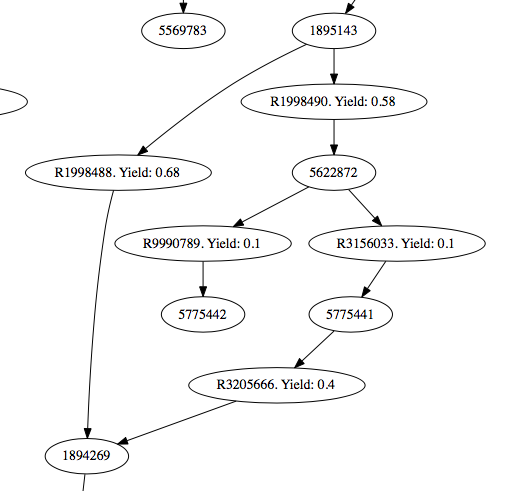
\includegraphics[scale=0.5]{Billeder/EvansCut.png}
\caption{}
\label{fig::EvansCut}
\end{figure}
Not only is it three reactions less but it also manages to avoid a reaction with a yield of 10\% (auto assigned). These three reactions also gives an explanation of the massive growth in the results.\\

\begin{figure}
\centering
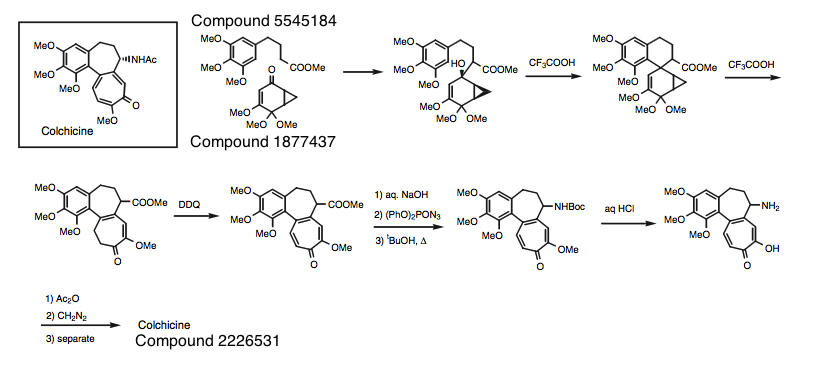
\includegraphics[scale=0.5, angle=90]{Synteseplaner/Colchicine/Evans.png}
\caption{Colchicine synthesis by D. A. Evans \cite{SynthesisPlans}}
\label{fig::Evans}
\end{figure}

\begin{figure}
\centering
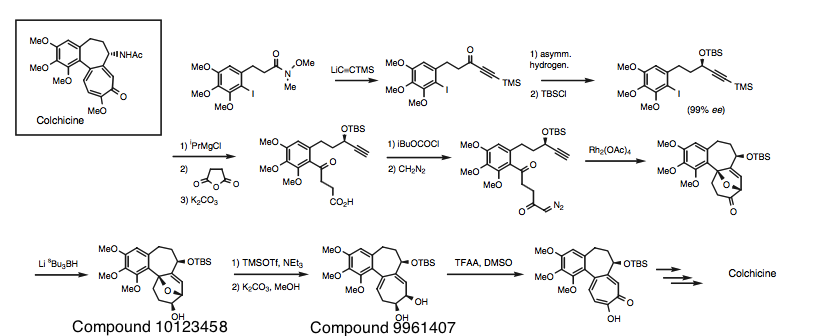
\includegraphics[scale=0.5, angle=90]{Synteseplaner/Colchicine/Schmalz.png}
\caption{Colchicine synthesis by H. G. Schmalz  \cite{SynthesisPlans}}
\label{fig::Schmalz}
\end{figure}

When it comes to plan 2, 4 and 5 it is harder to get a match on the synthesis plan by Schmalz (fig. \ref{fig::Schmalz}). Plan 2 matches on the compound 10123458 which is its starting compound, but in the original synthesis plan is close to the end. The following reactions and compounds does not match perfect with does depicted in Hoffman but the goal is a variant of Colchicine. Plan 4 and 5 both match on the compound 9961407 which is the second last compound in the original synthesis plan. Again it does not find perfect matches to the depictions of Hoffman, but also finds a way to Colchicine. The reason for the high results of 4 and 5 is because both plans have two reactions that have a yield of 10\% (auto assigned).\\
If the reactions in 3, 4 and 5 all had their yields from correct data, then they scores would have been much closer to each other, and not with the growth of approximately 7920 \%. 

\subsection{Dysidiolide}
There are in Hoffmann\cite{SynthesisPlans} four different plans for the compound Dysidiolide. These synthesis plans have been published in the following articles:
\begin{itemize}
\item
E. J. Corey, B. E. Roberts, J. Am. Chem. Soc. 1997, 119, 12425-12431.
\item
J. Boukouvalas, Y. X. Cheng, J. Robichaud, J. Org. Chem. 1998, 63, 228-229.
\item
S. R. Magnuson, L. Sepp-Lorenzino, N. Rosen, S. J. Danishefsky, J. Am. Chem.
Soc. 1998, 120, 1615-1616.
\item
D. Demeke, C. J. Forsyth, Org. Lett. 2000, 2, 3177-3179.
\item
R. Paczkowski, C. Maichle-Mössmer, M. E. Maier, Org. Lett. 2000, 2, 3967-3969.
\end{itemize}
The reason that there is five articles to four synthesis plans is because Forsyth and Maier is a combined synthesis plan. This time it was possible to retrieve all articles from Reaxys. The extracted hypergraph contained 119 compounds and 65 reactions. In the final generated graph there is 70 reactions. Once again this is because of the need to split the non-B-hyperedges.

\begin{figure}[H]
\centering
\includegraphics[scale=0.18]{Synteseplaner/Dysidiolide/Output.pdf}
\caption{Small version of the hypergraph. \href{Synteseplaner/Dysidiolide/Output.pdf}{Press here to see full pdf}}
\end{figure}

The created hypergraph have a high connectivity with close to none standalone reactions. The K-shortest algorithm was able to find 10 different synthesis plans.

\begin{table}[H]
\centering
\begin{tabular}{|r|r|r|}
\hline
Plan & Reactions & Starting weight \\ \hline
1 & \ref{Appendix::Dysidiolide1} & 6801,04 \\\hline
2 & \ref{Appendix::Dysidiolide2} & 8647,76 \\\hline
3 & \ref{Appendix::Dysidiolide3} & 10080,6 \\\hline
4 & \ref{Appendix::Dysidiolide4} & 12385,7 \\\hline
5 & \ref{Appendix::Dysidiolide5} & 12729 \\\hline
6 & \ref{Appendix::Dysidiolide6} & 15597,5 \\\hline
7 & \ref{Appendix::Dysidiolide7} & 21165,7 \\\hline
8 & \ref{Appendix::Dysidiolide8} & 22294,4 \\\hline
9 & \ref{Appendix::Dysidiolide9} & 23259 \\\hline
10 & \ref{Appendix::Dysidiolide10} & 27928,3 \\\hline
\end{tabular}
\caption{}
\label{tab::DysidiolideResults}
\end{table}

Plan 1-6 is generated from the compounds found in the synthesis plan from Danishefsky (fig. \ref{fig::Danishefsky}). Plan 1 and 2 goes all the way to the starting material (compound 5330688) depicted in Hoffmann, and are identical with the only exception of the second to last reaction that is changed from a 56\% reaction to a 45\% reaction. Plan 3-6 is the same plans as 1 and 2, except they go further away in the reactions including reactions and compounds that is not shown in Hoffman. The differences between these plans is the second to last reaction, and that there is a possibility to skip two reactions between compound 1738097 and compound 1815228 by using reaction R5142034.\\

Plan 7 and 9 are both from Coreys synthesis plan (fig. \ref{fig::Corey}. The matching with the plan in Hoffmann ends at compound 8166687 that is to found almost at the top of the plan. The difference between the plans is that it is possible to skip two reactions at the end of the synthesis plan. Reaction R8540393 was original a non-B-hyperedge that both lead to compound 8168305 and the compound 8168306, but have been split, so by using the new reaction R10207847 that leads to  compound 8168306 we can skip the steps that it takes for compound 8168305 to become compound 8168306.\\

Both plan 8 and 10 are from Forsyth and Maiers synthesis plan (fig. \ref{fig::Forsyth}). It have been possible to match the plans until compound 8633878, which resides in the middle of the synthesis plans found. The last two steps of the synthesis plan is identical to the plans from Danishefsky. Just as with Danishefsky the second to last reaction can be changed, and this is what leads to the two different plans.\\

There is a small jump in cost between plan 6 and plan 7. One reason for this could be that the first reaction of plan 7 and 9 is R5075479 which has an auto assigned yield of 10\%. What goes for plan 8 and 10, is it assumed that the length of the plan alone is responsible for the cost of the plan.\\ 
One might ask: Where is the plan generated by the article of J. Boukouvalas? The starting compound 3543574 is 
found at the top of a small sub-hypergraph that is cut off from the rest of the hypergraph, which leads me to think that there have been a possible multi-step reaction linking it together with the rest of the hypergraph. But since there is no link there is no path from $s$ to $t$ and therefore no synthesis plan.
\begin{figure}
\centering
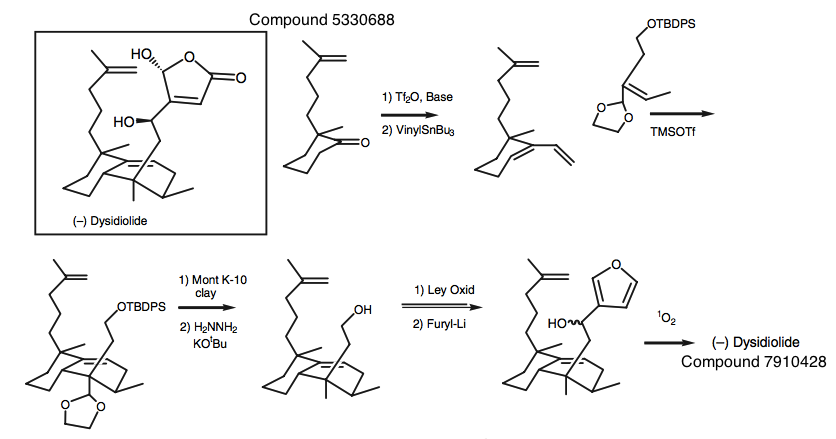
\includegraphics[scale=0.5, angle=90]{Synteseplaner/Dysidiolide/Danishefsky.png}
\caption{Dysidiolide synthesis by S. J. Danishefsky \cite{SynthesisPlans}}
\label{fig::Danishefsky}
\end{figure}

\begin{figure}
\centering
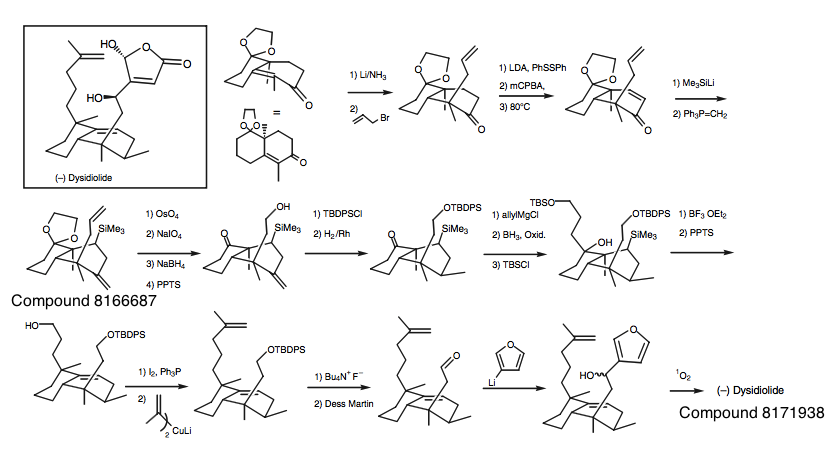
\includegraphics[scale=0.5, angle=90]{Synteseplaner/Dysidiolide/Corey.png}
\caption{Dysidiolide synthesis by E. J. Corey  \cite{SynthesisPlans}}
\label{fig::Corey}
\end{figure}

\begin{figure}
\centering
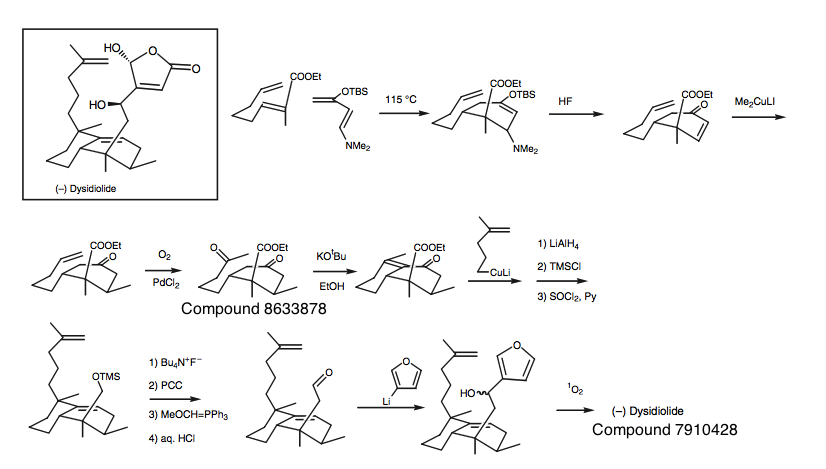
\includegraphics[scale=0.5, angle=90]{Synteseplaner/Dysidiolide/Forsyth.png}
\caption{Dysidiolide synthesis by Forsyth and Maier \cite{SynthesisPlans}}
\label{fig::Forsyth}
\end{figure}

\subsection{Asteriscanolide}
There are in Hoffmann\cite{SynthesisPlans} four different plans for the compound Asteriscanolide. These synthesis plans have been published in the following articles:
\begin{itemize}
\item
M. E. Krafft, Y. Y. Cheung, C. A. Juliano-Capucao, Synthesis 2000, 1020-1026.
\item
M. E. Krafft, Y. Y. Cheung, K. A. Abboud, J. Org. Chem. 2001, 66, 7443-7448.
\item
L.A.Paquette, J. Tae, M. P. Arrington, A. H. Sadoun, J. Am. Chem. Soc. 2000,122,
2742-2748.
\item
P. A. Wender, N. C. Ihle, C. R .D. Correia, J. Am. Chem. Soc. 1988, 110,5904-5906.
\item
J. Limanto, M. L. Snapper, J. Am. Chem. Soc. 2000, 122, 8071-8072.
\end{itemize}
The two first articles describe the same synthesis plan. The XML file for L. A. Paquette's article did not contain the final goal compound Asteriscanolide as one of its listed compounds. The articles reactions and compounds were however still added to the creation of the hypergraph.
The extracted hypergraph contained 104 compounds and 49 reactions. In the final generated graph there is 50 reactions. Again, this is because of the need to split the non-B-hyperedges.

\begin{figure}
\centering
\includegraphics[scale=0.17, angle=90]{Synteseplaner/Asteriscanolide/Output.pdf}
\caption{Small version of the hypergraph. \href{Synteseplaner/Asteriscanolide/Output.pdf}{Press here to see full pdf}}
\label{fig::AsteriscanolideGraph}
\end{figure}

Considering that this graph (fig. \ref{fig::AsteriscanolideGraph}) was created using only four different articles, it is quite spares. There is only two sub-hypergraphs, that have a potential path length longer than four reactions, and only one of these contains a target compound. The K-shortest algorithm was able to find 3 different synthesis plans. 

\begin{table}[H]
\centering
\begin{tabular}{|r|r|r|}
\hline
Plan & Reactions & Starting weight \\ \hline
1 & \ref{Appendix::Asteriscanolide1} & 649,346 \\\hline
2 & \ref{Appendix::Asteriscanolide2} & 5175,63 \\\hline
3 & \ref{Appendix::Asteriscanolide3} & 13549,2 \\\hline
\end{tabular}
\caption{}
\end{table}
Plan 1 is a part of the synthesis plan from Wender (fig. \ref{fig::Wender}). The found plan matches step by step the last three reactions of the original plan, and stops at compound 6198015.\\
Plan 2 is the last part of the synthesis plan from Snapper (fig. \ref{fig::Snapper}). Once again it matches step by step the reactions of the original plan. This time it reaches four reactions backwards until it stops at compound 10443050.\\
Plan 3 is the longest of the synthesis plans found, and matches that of Krafft (fig. \ref{fig::Krafft}). Some of the steps in the found plan are intermediate steps when looking at the description in Hoffmann. The plan found could be matched until compound 8546300.\\

As expected there were no plan for the article by L. A. Paquette, since the goal compound was not included in the XML file. The increase in scores on plan 2 and 3 is because the first reaction of each plan uses an auto assigned yield of 10\%. \\

\begin{figure}
\centering
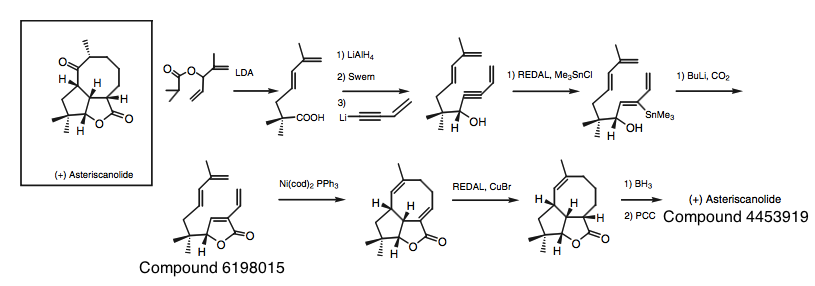
\includegraphics[scale=0.5, angle=90]{Synteseplaner/Asteriscanolide/Wender.png}
\caption{Asteriscanolide synthesis by P. A. Wender \cite{SynthesisPlans}}
\label{fig::Wender}
\end{figure}

\begin{figure}
\centering
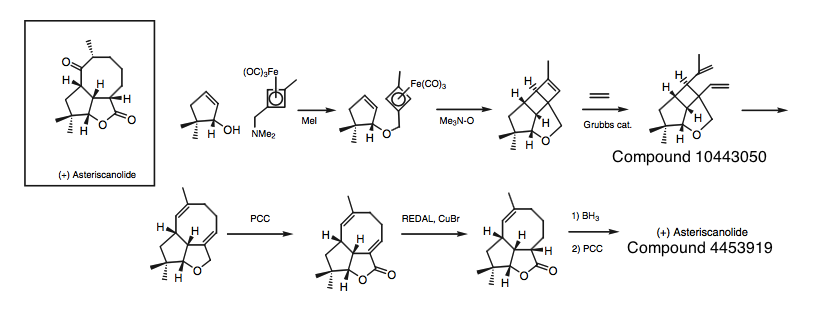
\includegraphics[scale=0.5, angle=90]{Synteseplaner/Asteriscanolide/Snapper.png}
\caption{Asteriscanolide synthesis by M. L. Snapper  \cite{SynthesisPlans}}
\label{fig::Snapper}
\end{figure}

\begin{figure}
\centering
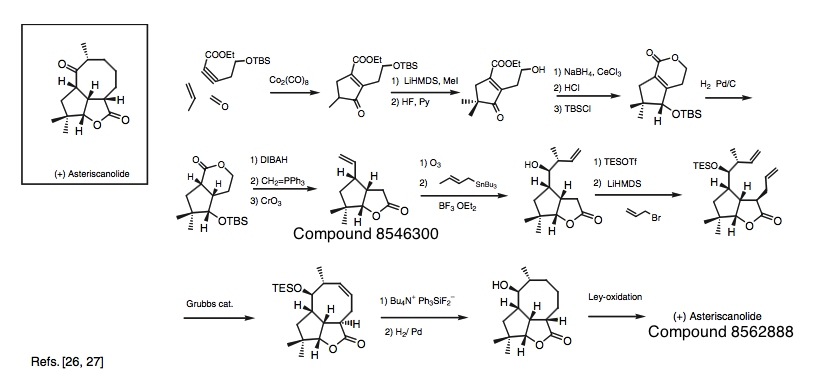
\includegraphics[scale=0.5, angle=90]{Synteseplaner/Asteriscanolide/Krafft.png}
\caption{Asteriscanolide synthesis by M. E. Krafft \cite{SynthesisPlans}}
\label{fig::Krafft}
\end{figure}

\subsection{Lepadiformine}
There are in Hoffmann\cite{SynthesisPlans} four different plans for the compound Lepadiformine. These synthesis plans have been published in the following articles:
\begin{itemize}
\item
T. J. Greshock, R. L. Funk, Org. Lett. 2001, 3, 3511-3514.
\item
P. Sun, C. Sun, S. M. Weinreb, J. Org. Chem. 2002, 67, 4337-4345.
\item
S. M. Weinreb, Acc. Chem. Res. 2003, 36, 59–65.
\item
H. Abe, S. Aoyagi, C. Kibayashi, Angew. Chem., Int. Ed. 2002, 41, 3017-3020.
(Angew. Chem. 2002, 114, 3143-3146).
\item
C. Kibayashi, S. Aoyagi, H. Abe, Bull. Chem. Soc. Jpn. 2003, 76, 2059-2074.
\item
H. Abe, S. Aoyagi, C. Kibayashi, J. Am. Chem. Soc. 2005, 127, 1473-1480.
\item
Proposal by the R. W. Hoffmann Group, 2001.
\end{itemize}
The three articles by Kibayashi all describe the same synthesis plan. The synthesis plan that comes from "Proposal by the R. W. Hoffmann Group" was not to be found on Reaxys, since there was no precise keywords or documents to search for.
The extracted hypergraph contained 94 compounds and 56 reactions. In the final generated graph there is 60 reactions due to non-B-hyperedges conflict resolving. 

\begin{figure}
\centering
\includegraphics[scale=0.17, angle=90]{Synteseplaner/Lepadiformine/Output.pdf}
\caption{Small version of the hypergraph. \href{Synteseplaner/Lepadiformine/Output.pdf}{Press here to see full pdf}}
\label{fig::LepadiformineGraph}
\end{figure}

The created hypergraph (fig. \ref{fig::LepadiformineGraph}) has the highest connectivity among all the experiments. However, since both goal compounds are found in the right sub-hypergraph there would be not much variation of the found synthesis plans. The K-shortest algorithm was able to find 6 different synthesis plans. 

\begin{table}[H]
\centering
\begin{tabular}{|r|r|r|}
\hline
Plan & Reactions & Starting weight \\ \hline
1 & \ref{Appendix::Lepadiformine1} & 841,29 \\\hline
2 & \ref{Appendix::Lepadiformine2} & 1061,41 \\\hline
3 & \ref{Appendix::Lepadiformine3} & 1129,16 \\\hline
4 & \ref{Appendix::Lepadiformine4} & 5138,44 \\\hline
5 & \ref{Appendix::Lepadiformine5} & 7629,88 \\\hline
6 & \ref{Appendix::Lepadiformine6} & 8116,89 \\\hline
\end{tabular}
\caption{}
\end{table}

Plan 1 is surprisingly not the shortest of the found synthesis plans. The origin of the plan is the synthesis plan from Funk (fig. \ref{fig::Funk}). We are able to follow the synthesis plan two reactions backwards until we hit the compound 8949596. 

Plan 2 and 3 are the longest of the found synthesis plans. They come from the synthesis plan by Kibayashi (fig. \ref{fig::Kibayashi}). Even though the synthesis plan found contains more reactions than the one depicted in Hoffmann, it is the same. The starting compound 9367668 is the second compound of the synthesis plan shown in Hoffmann. The two plans differ in the last reaction. Plan 2 uses a reaction with a yield of 100\% and plan 3 uses a reaction with a yield of 94\%.

Plan 4, 5 and 6 are parts of the synthesis plan by Weinreb (fig. \ref{fig::Weinreb}). There is close to no match between the compounds shown in Hoffmann, but it is known that the synthesis plans found origins from Weinreb because the reactions are in the XML files. The furthest back the plans can be shown to fit is compound 9223049, which is the second to last compound in the synthesis plan shown in Hoffmann. This compound is part of plan 5 and 6.\\

The rise in cost between 3 and 4 is once again due to an auto assign of yield. Plan 4, 5 and 6, all start with a reaction with a yield of 10\%.

\begin{figure}
\centering
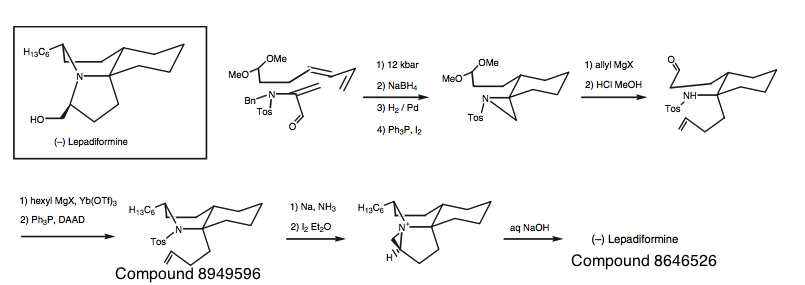
\includegraphics[scale=0.5, angle=90]{Synteseplaner/Lepadiformine/Funk.png}
\caption{Lepadiformine synthesis by R. L. Funk \cite{SynthesisPlans}}
\label{fig::Funk}
\end{figure}

\begin{figure}
\centering
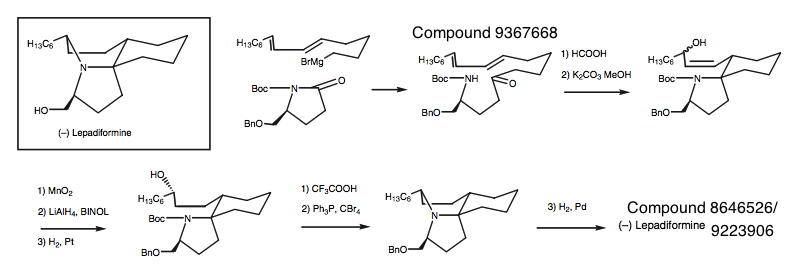
\includegraphics[scale=0.5, angle=90]{Synteseplaner/Lepadiformine/Kibayashi.png}
\caption{Lepadiformine synthesis by C. Kibayashi  \cite{SynthesisPlans}}
\label{fig::Kibayashi}
\end{figure}

\begin{figure}
\centering
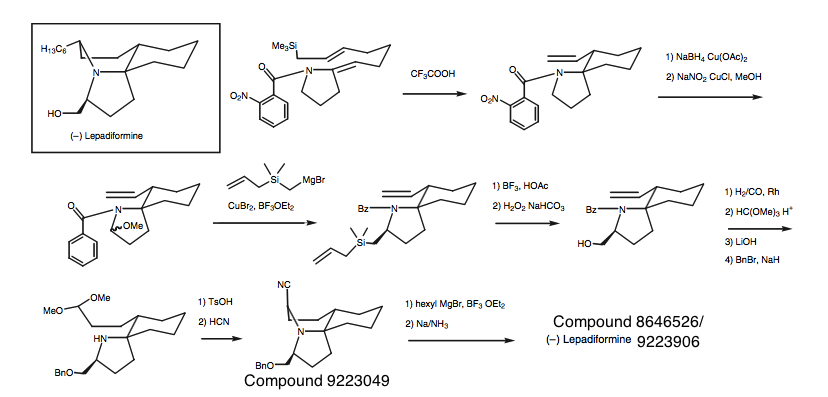
\includegraphics[scale=0.5, angle=90]{Synteseplaner/Lepadiformine/Weinreb.png}
\caption{Lepadiformine synthesis by S. M. Weinreb \cite{SynthesisPlans}}
\label{fig::Weinreb}
\end{figure}


\subsection{General notes}
As the reader might have noticed, all the found synthesis plans are close to being completely linear. This is because the hypergraphs that the algorithms have work with were based on already known synthesis plans. This made the hypergraphs goal oriented. As described in the following section, Future work, it would be interesting to be able to expand on already known hypergraphs. This would broaden the search space and probably show synthesis plans with a larger breath, looking more like a balanced tree instead of a linked list.

\subsection{Evaluation of results}
By using the already known synthesis plans of specific compounds it have been possible to generate hypergraphs on which the K-best algorithm could run. The results have been overall satisfying. It was possible to distinguish exactly from which known synthesis plans the newly found ones originated, even if there never was a perfect match. 

\section{Future work}
\label{sec::FutureWork}
This section describes possible correction of errors that was discovered close to deadline or missing features of the program. It also contains ideas for further work on the data from Beilstein.
\subsection{Expanding}
The idea of expanding is to have either a compound or an existing synthesis plan and to expand on these. If we have a single target compound, it would be possible to expand step-wise from that compound. By doing this we are able to find all compounds from which it is possible to create the target by using only $B$ reactions. Once the expansion have been made the K-shortest algorithm could run using all compounds of the hypergraph that have a in-degree = 0 as staring compounds.
\begin{figure}[H]
\centering
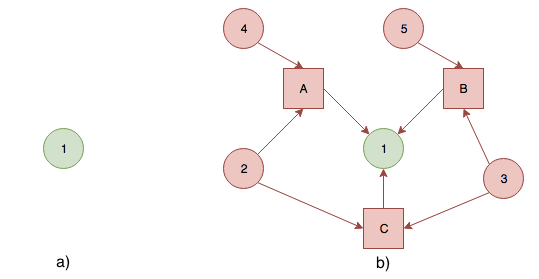
\includegraphics[scale=0.5]{Billeder/TestOfExpansion1.png}
\caption{\textbf{a)} The target compound. \\ \textbf{b)} After a single expansion from target compound}
\end{figure} 

\begin{figure}[H]
\centering
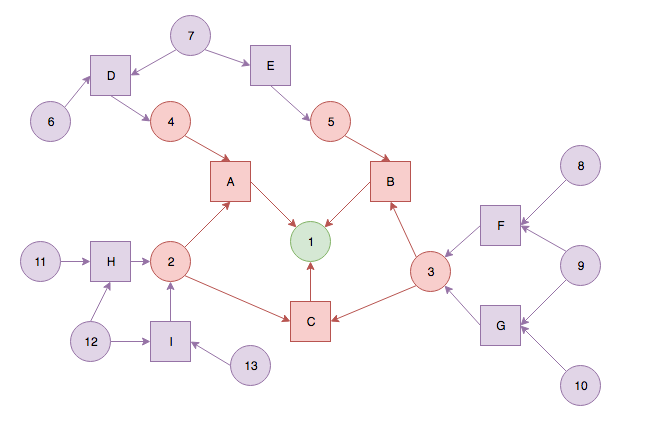
\includegraphics[scale=0.5]{Billeder/TestOfExpansion2.png}
\caption{The hypergraph after a two expansions from target compound}
\end{figure} 
If we instead would have a existing synthesis plan, or perhaps a set of synthesis plans, from a published article. We could expand on each of the compounds in the plan. Even though we use already known reactions the reactions that are added might reveal connections that have not been used before to create that specific target compound. If we look at fig. \ref{fig::ExpansionOfPath} we can see that the expansion of the known synthesis plan have revealed a new path from compound 3 to the target compound 1 through the reactions G and F. It also reveals another way of creating compound 3 with the use of reaction H. If reaction H have a better yield than reaction C, it might result in a better plan. The author of the synthesis plan could simply have forgotten about reaction H or he did not know that a new reaction had been discovered, and therefore only thought that C was an option. 
\begin{figure}[H]
\centering
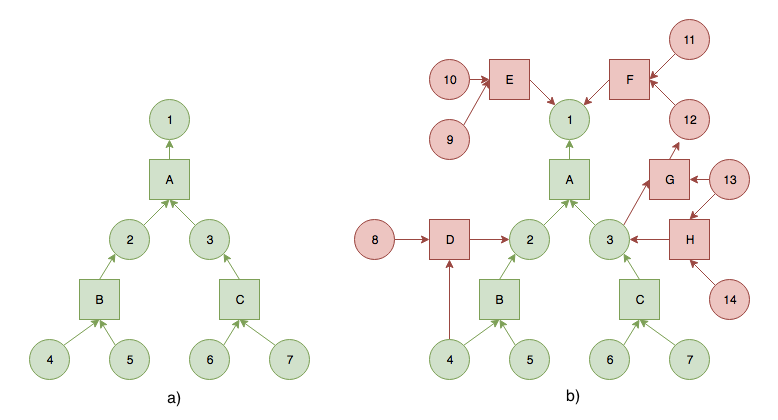
\includegraphics[scale=0.5]{Billeder/ExpansionOfPath.png}
\caption{\textbf{a)} A hypergraph made from an existing synthesis plan. \textbf{b)} A single step expansion of the given synthesis plan.}
\label{fig::ExpansionOfPath}
\end{figure}
\subsection{Error handling}
That the program throws a segmentation fault when the dynamic approach is used on a hypergraph with cycles, is of course not preferable. It should however use the visited attribute of the CompoundNodes for cycle detection. If an already visited node is visited again it should abort the algorithm, print an error messsage so that the user may know why the algorithm fails.\\
The problem with STB-Dijkstra in test 4 \ref{sec::testing} should be investigate so that the problem can be fixed. As mentioned before it only seems to happen in the tests made by SynthWorker and in a hypergraph with many equally good paths, but should non the less be fixed.
\subsection{Specific start weight}
At the time of deadline, the results of the shortest path algorithms is the accumulated weight of the starting materials. This is a good way of determining if a path is better than another. It would however be a good thing to know how much of each of the individual staring materials should be used to create the target compound, for pratical purposes. To calculate the individual weight of the staring materials, we would need to implement a Depth-First-Search inspired algorithm that starts in the goal compound and traverses the synthesis plan towards the starting materials. For each reaction, $e$, it comes through on its path, the cost of $H(e)$ is divided with the retroyield ($1/yield_e$) and passed on to the nodes in $T(e)$ as the "inverted cost". When the algorithm hits a starting compound it divides the cost of the goal compound with the inverted cost of the staring material found by the DFS and multiplies it with the molecular weight of the starting compound.
\begin{figure}[H]
\centering
\includegraphics[scale=0.5]{Billeder/StartingMaterialCalculation.png}
\end{figure}
If we use the example above we can see that the result of the shortest path algorithms were 21,42857. By calculating the inverse cost from the target and down to the staring compounds 4, 5, 6, 7 leads to the following starting weights of the compounds:
\begin{align}
\{4,5\} &= (21,42857/7,4999) \cdot 2 \approx 5,71436\\
\{6,7\} &= (21,42857/8,571428) \cdot 2 = 5
\end{align}
By dividing these results with the molecular weight of the compounds, we would get how many times of each starting compound we would need to create a single target compound.
\subsection{Pricing}
There is also the possibility of adding new attributes to the structure. It would be possible to find all those compounds which can be bought on the open market, and add a price to each of the compounds. The reactions would then need to have a price in the form of lab costs, so that when a reaction is made, it takes into consideration that there is a potential cost to equipment and/or personnel.\\
Each compound that have a market price would become a starting material, since it would be possible just to buy the compound instead of making it. The shortest path algorithm would now find the $K$ shortest synthesis plans that not only gives the highest yield, but also takes into consideration if it would be cheaper to use a longer synthesis plan, with more reactions, to make the same amount of the target compound. An example of this would be that the work cost in Germany is much higher than in China. This means that it could be profitable for the chinese to buy cheaper compounds and make the more expensive compounds themselves, whereas the german scientists would find it more profitable to start at more complex compound, since it would be more profitable to buy the compound instead of making it themselves from scratch.
\section{Conclusion}
\label{sec::Conclusion}
By using a hypergraph consisting of chemical compounds and chemical reaction we have shown that it is possible to enumerate the $K$-best synthesis plans given a set of goal compounds and a set of starting materials. To enumerate the $K$-best plans a modification of Yen's algorithm is used alongside a shortest path algorithm. The use of an overlay to remove the costly function of copying the whole hypergraph when changes are made, have been proposed in this thesis.\\ 
If the hypergraph is acyclic it is possible to list the $K$-best plans in $\mathcal{O}(K \cdot |V| \cdot (|V|+|E|))$ using a dynamic approach\cite{Carsten} and the appropriate cost function.\\
Should the hypergraph be cyclic, there is the possibility of using the STB-Dijkstra\cite{Nielsen} algorithm instead. The algorithm is able to enumerate the $K$-best plans in 
$\mathcal{O}(K \cdot |V| \cdot (|E|\ log_2 (|V)| + size(h)))$. In the attempt of decreasing the run time of STB-Dijkstra it have been shown that by using the dynamic approach to mark all reactions it traverses, it is possible to prune the hypergraph and thereby reducing the search space of the STB-Dijkstra.\\
To show the practical use of the $K$-best algorithm, experiments were made to try to recreate already known synthesis plans. The idea was to take the compounds and reactions of already known and documented synthesis plans from the Beilstein database in Leipzig and see if the K-best algorithm could reproduce them. The synthesis plans chosen came from the book "Elements of Synthesis Planning" by R. W. Hoffmann. In this book the synthesis plans were depicted and had references to the articles from which they originated. The compounds were: Strychnine, Colchicine, Dysidiolide, Asteriscanolide and Lepadiformine. The results were very satisfying since almost all synthesis plans were reproduced. That some of the synthesis plans were not found is most likely due to imperfect data. Some of the hypergraphs generated were sparse and had multiple unlinked sub-hypergraphs, making it hard to find the full length of the synthesis plans.\\
It would be interesting to be able to expand on the synthesis plan already known or from a given target compound. This could lead to new unseen synthesis plans that might be better (or worse) than those already known. This would however need an direct access to the Beilstein database. It would also be interesting to use prices of compounds and actual work cost as another minimizing objective instead of weight and yield.

\newpage

\printbibliography[type=book, title={Books}]
\printbibliography[type=article, title={Articles}]
\printbibliography[nottype=book, nottype=article, title={Other}]

\newpage
\appendix
\addtocontents{toc}{\protect\setcounter{tocdepth}{1}}
\section{Test Graphs}

\subsection{Thesis Graph}
\centering
\includegraphics[scale=0.4]{TestGrafer/ThesisTest.pdf}
\label{Appendix::ThesisGraph}

\subsection{Paper Graph}
\centering
\includegraphics[scale=0.4]{TestGrafer/PaperTest.pdf}
\label{Appendix::Paper Graph}

\subsection{Deadend Graph}
\centering
\includegraphics[scale=0.4]{TestGrafer/Deadend.pdf}
\label{Appendix::DeadEnd Graph}

\subsection{Cycle Graph}
\centering
\includegraphics[scale=0.4]{TestGrafer/CycleTest.pdf}
\label{Appendix::Cycle Graph}

\section{Rojin Tests}
\subsection{Rojin Test 1}
\centering
\includegraphics[scale=0.4]{RojinGrafer/Test1.pdf}
\label{Appendix::Rojin1}

\subsection{Rojin Test 2}
\centering
\includegraphics[scale=0.4, angle=90]{RojinGrafer/Test2.pdf}
\label{Appendix::Rojin2}

\subsection{Rojin Test 3}
\includegraphics[scale=0.4]{RojinGrafer/Test3.pdf}
\label{Appendix::Rojin3}

\subsection{Rojin Test 4}
\begin{flushleft}
Hypergraph to big to be on page. \href{RojinGrafer/test4.pdf}{Press here to see pdf}.
\label{Appendix::Rojin4}
\end{flushleft}

\subsection{Rojin Test 5}
\begin{flushleft}
Hypergraph to big to be on page. \href{RojinGrafer/test5.pdf}{Press here to see pdf}.
\end{flushleft}
\label{Appendix::Rojin5}

\subsection{Rojin Test 6}
\begin{flushleft}
Hypergraph to big to be on page. \href{RojinGrafer/test6.pdf}{Press here to see pdf}.
\end{flushleft}
\label{Appendix::Rojin6}

\subsection{Rojin Test 7 }
\begin{flushleft}
Hypergraph to big to be converted from dot to pdf. Hypergraph omited.
\end{flushleft}
\label{Appendix::Rojin7}

\section{Synthesis Plans}
\subsection{Strychnine plan 1}
\centering
\includegraphics[scale=0.4]{Synteseplaner/Strychnine/plan1.pdf}
\label{Appendix::Strychnine1}

\subsection{Strychnine plan 2}
\centering
\includegraphics[scale=0.4]{Synteseplaner/Strychnine/plan2.pdf}
\label{Appendix::Strychnine2}

\subsection{Strychnine plan 3}
\centering
\includegraphics[scale=0.4]{Synteseplaner/Strychnine/plan3.pdf}
\label{Appendix::Strychnine3}


\subsection{Strychnine plan 4}
\centering
\includegraphics[scale=0.4]{Synteseplaner/Strychnine/plan4.pdf}
\label{Appendix::Strychnine4}

\subsection{Strychnine plan 5}
\centering
\includegraphics[scale=0.4]{Synteseplaner/Strychnine/plan5.pdf}
\label{Appendix::Strychnine5}


\subsection{Strychnine plan 6}
\centering
\includegraphics[scale=0.4]{Synteseplaner/Strychnine/plan6.pdf}
\label{Appendix::Strychnine6}

\subsection{Strychnine plan 7}
\centering
\includegraphics[scale=0.4]{Synteseplaner/Strychnine/plan7.pdf}
\label{Appendix::Strychnine7}


\subsection{Strychnine plan 8}
\centering
\includegraphics[scale=0.4]{Synteseplaner/Strychnine/plan8.pdf}
\label{Appendix::Strychnine8}

\subsection{Strychnine plan 9}
\centering
\includegraphics[scale=0.4]{Synteseplaner/Strychnine/plan9.pdf}
\label{Appendix::Strychnine9}

\subsection{Strychnine plan 10}
\centering
\includegraphics[scale=0.4]{Synteseplaner/Strychnine/plan10.pdf}
\label{Appendix::Strychnine10}

\subsection{Strychnine plan 11}
\centering
\includegraphics[scale=0.4]{Synteseplaner/Strychnine/plan11.pdf}
\label{Appendix::Strychnine11}

\subsection{Strychnine plan 12}
\centering
\includegraphics[scale=0.4]{Synteseplaner/Strychnine/plan12.pdf}
\label{Appendix::Strychnine12}

\subsection{Strychnine plan 13}
\centering
\includegraphics[scale=0.4]{Synteseplaner/Strychnine/plan13.pdf}
\label{Appendix::Strychnine13}

\subsection{Strychnine plan 14}
\centering
\includegraphics[scale=0.4]{Synteseplaner/Strychnine/plan14.pdf}
\label{Appendix::Strychnine14}

\subsection{Strychnine plan 15}
\centering
\includegraphics[scale=0.4]{Synteseplaner/Strychnine/plan15.pdf}
\label{Appendix::Strychnine15}

\subsection{Strychnine plan 16}
\centering
\includegraphics[scale=0.4]{Synteseplaner/Strychnine/plan16.pdf}
\label{Appendix::Strychnine16}

\subsection{Colchicine plan 1}
\centering
\includegraphics[scale=0.4]{Synteseplaner/Colchicine/plan1.pdf}
\label{Appendix::Colchicine1}

\subsection{Colchicine plan 2}
\centering
\includegraphics[scale=0.4]{Synteseplaner/Colchicine/plan2.pdf}
\label{Appendix::Colchicine2}

\subsection{Colchicine plan 3}
\centering
\includegraphics[scale=0.4]{Synteseplaner/Colchicine/plan3.pdf}
\label{Appendix::Colchicine3}

\subsection{Colchicine plan 4}
\centering
\includegraphics[scale=0.4]{Synteseplaner/Colchicine/plan4.pdf}
\label{Appendix::Colchicine4}

\subsection{Colchicine plan 5}
\centering
\includegraphics[scale=0.4]{Synteseplaner/Colchicine/plan5.pdf}
\label{Appendix::Colchicine5}

\subsection{Dysidiolide plan 1}
\centering
\includegraphics[scale=0.43]{Synteseplaner/Dysidiolide/plan1.pdf}
\label{Appendix::Dysidiolide1}

\subsection{Dysidiolide plan 2}
\centering
\includegraphics[scale=0.43]{Synteseplaner/Dysidiolide/plan2.pdf}
\label{Appendix::Dysidiolide2}

\subsection{Dysidiolide plan 3}
\centering
\includegraphics[scale=0.34]{Synteseplaner/Dysidiolide/plan3.pdf}
\label{Appendix::Dysidiolide3}

\subsection{Dysidiolide plan 4}
\centering
\includegraphics[scale=0.3]{Synteseplaner/Dysidiolide/plan4.pdf}
\label{Appendix::Dysidiolide4}

\subsection{Dysidiolide plan 5}
\centering
\includegraphics[scale=0.35]{Synteseplaner/Dysidiolide/plan5.pdf}
\label{Appendix::Dysidiolide5}

\subsection{Dysidiolide plan 6}
\centering
\includegraphics[scale=0.3]{Synteseplaner/Dysidiolide/plan6.pdf}
\label{Appendix::Dysidiolide6}

\subsection{Dysidiolide plan 7}
\centering
\includegraphics[scale=0.27]{Synteseplaner/Dysidiolide/plan7.pdf}
\label{Appendix::Dysidiolide7}

\subsection{Dysidiolide plan 8}
\centering
\includegraphics[scale=0.2]{Synteseplaner/Dysidiolide/plan8.pdf}
\label{Appendix::Dysidiolide8}

\subsection{Dysidiolide plan 9}
\centering
\includegraphics[scale=0.25]{Synteseplaner/Dysidiolide/plan9.pdf}
\label{Appendix::Dysidiolide9}

\subsection{Dysidiolide plan 10}
\centering
\includegraphics[scale=0.2]{Synteseplaner/Dysidiolide/plan10.pdf}
\label{Appendix::Dysidiolide10}

\subsection{Asteriscanolide plan 1}
\centering
\includegraphics[scale=0.4]{Synteseplaner/Asteriscanolide/plan1.pdf}
\label{Appendix::Asteriscanolide1}

\subsection{Asteriscanolide plan 2}
\centering
\includegraphics[scale=0.4]{Synteseplaner/Asteriscanolide/plan2.pdf}
\label{Appendix::Asteriscanolide2}

\subsection{Asteriscanolide plan 3}
\centering
\includegraphics[scale=0.4]{Synteseplaner/Asteriscanolide/plan3.pdf}
\label{Appendix::Asteriscanolide3}

\subsection{Lepadiformine plan 1}
\centering
\includegraphics[scale=0.4]{Synteseplaner/Lepadiformine/plan1.pdf}
\label{Appendix::Lepadiformine1}

\subsection{Lepadiformine plan 2}
\centering
\includegraphics[scale=0.4]{Synteseplaner/Lepadiformine/plan2.pdf}
\label{Appendix::Lepadiformine2}

\subsection{Lepadiformine plan 3}
\centering
\includegraphics[scale=0.4]{Synteseplaner/Lepadiformine/plan3.pdf}
\label{Appendix::Lepadiformine3}

\subsection{Lepadiformine plan 4}
\centering
\includegraphics[scale=0.4]{Synteseplaner/Lepadiformine/plan4.pdf}
\label{Appendix::Lepadiformine4}

\subsection{Lepadiformine plan 5}
\centering
\includegraphics[scale=0.4]{Synteseplaner/Lepadiformine/plan5.pdf}
\label{Appendix::Lepadiformine5}

\subsection{Lepadiformine plan 6}
\centering
\includegraphics[scale=0.4]{Synteseplaner/Lepadiformine/plan6.pdf}
\label{Appendix::Lepadiformine6}
\end{document}